% =====================================================================
%  RELAZIONE FINALE - Corso di Manutenzione Preventiva A.A. 2025/2026
%  Esacottero DJI F550 - Pixhawk 6X - PX4
%
%  Compilazione:  pdflatex main && pdflatex main   (due passate per ToC)
%  Template TEMPORANEO - vedi relazione/linee-guida.md
% =====================================================================
\documentclass[11pt,a4paper,oneside]{report}
% =====================================================================
%  Preambolo / template TEMPORANEO della relazione
%  Corso di Manutenzione Preventiva - A.A. 2025/2026 - Esacottero F550
%  NB: template provvisorio, da rifinire quando il docente fissa il formato.
% =====================================================================

\usepackage[T1]{fontenc}
\usepackage[utf8]{inputenc}
\usepackage{lmodern}
\usepackage{textcomp}
\usepackage{csquotes}
\usepackage{microtype}

% --- Lingua ---
% Usa babel italiano se disponibile (pacchetto Debian: texlive-lang-italian);
% altrimenti ripiega su babel inglese con etichette/data in italiano, cos\`i la
% compilazione non si blocca. Per la sillabazione italiana corretta installare:
%   sudo apt-get install texlive-lang-italian
\IfFileExists{italian.ldf}{%
  \usepackage[italian]{babel}%
}{%
  \usepackage[english]{babel}%
  \addto\captionsenglish{%
    \renewcommand{\contentsname}{Indice}%
    \renewcommand{\chaptername}{Capitolo}%
    \renewcommand{\appendixname}{Appendice}%
    \renewcommand{\tablename}{Tabella}%
    \renewcommand{\figurename}{Figura}%
    \renewcommand{\listtablename}{Elenco delle tabelle}%
    \renewcommand{\listfigurename}{Elenco delle figure}%
    \renewcommand{\bibname}{Riferimenti}}%
  \AtBeginDocument{\renewcommand{\today}{\number\day~\ifcase\month\or gennaio\or
    febbraio\or marzo\or aprile\or maggio\or giugno\or luglio\or agosto\or
    settembre\or ottobre\or novembre\or dicembre\fi~\number\year}}%
}

% --- Geometria pagina ---
\usepackage{amssymb}
\usepackage[a4paper,top=2.6cm,bottom=2.6cm,left=2.7cm,right=2.7cm]{geometry}
\usepackage{setspace}
\onehalfspacing

% --- Tabelle ---
\usepackage{booktabs}
\usepackage{tabularx}
\usepackage{array}
\usepackage{longtable}
\newcolumntype{L}[1]{>{\raggedright\arraybackslash}p{#1}}
\newcolumntype{C}[1]{>{\centering\arraybackslash}p{#1}}

% --- Figure ---
\usepackage{graphicx}
\graphicspath{{img/}{../img/}{../plot/}{../plot/imu/}{../plot/esc/}{../plot/batteria/}{../plot/incidente/}}
\usepackage{float}
\usepackage[font=small,labelfont=bf,margin=1em]{caption}

% --- Colori e box ---
\usepackage{xcolor}
\definecolor{blunavy}{HTML}{1F3A5F}
\definecolor{griginochiaro}{HTML}{F2F4F7}
\definecolor{accentoblu}{HTML}{2D6CDF}
\usepackage[most]{tcolorbox}

% Box generico per note/avvertenze
\newtcolorbox{notabox}[1][Nota]{
  colback=griginochiaro, colframe=blunavy, fonttitle=\bfseries,
  title=#1, boxrule=0.6pt, arc=2pt, left=4pt, right=4pt, top=3pt, bottom=3pt}

% Box checklist
\newtcolorbox{checklistbox}[1][Checklist]{
  colback=white, colframe=accentoblu, fonttitle=\bfseries\color{white},
  coltitle=white, title=#1, boxrule=0.8pt, arc=2pt}

% --- Liste ---
\usepackage{enumitem}
\setlist{itemsep=2pt,topsep=3pt}

% --- Intestazioni ---
\usepackage{fancyhdr}
\pagestyle{fancy}
\fancyhf{}
\fancyhead[L]{\small\nouppercase{\leftmark}}
\fancyhead[R]{\small Manutenzione Preventiva --- F550}
\fancyfoot[C]{\thepage}
\renewcommand{\headrulewidth}{0.4pt}

% Titoli capitolo/sezione coerenti col colore
\usepackage{titlesec}
\titleformat{\chapter}[display]
  {\normalfont\huge\bfseries\color{blunavy}}
  {\chaptertitlename\ \thechapter}{14pt}{\Huge}
\titleformat{\section}
  {\normalfont\Large\bfseries\color{blunavy}}{\thesection}{1em}{}
\titleformat{\subsection}
  {\normalfont\large\bfseries\color{blunavy!85}}{\thesubsection}{1em}{}

% --- Link ---
\usepackage[hidelinks]{hyperref}
\hypersetup{
  colorlinks=true, linkcolor=blunavy, citecolor=blunavy,
  urlcolor=accentoblu, pdftitle={Relazione Manutenzione Preventiva F550}}

% --- Comando segnaposto figura (img/ ancora da popolare) ---
% Uso: \figurasegnaposto{didascalia}{tipo}{label}
\newcommand{\figurasegnaposto}[3]{%
  \begin{figure}[H]\centering
  \fbox{\begin{minipage}[c][3.2cm][c]{0.8\linewidth}\centering
    \textit{[Segnaposto figura --- #2]}\\[2pt]\small #1
  \end{minipage}}
  \caption{#1}\label{#3}
  \end{figure}}

% Acronimo TODO visibile in bozza
\newcommand{\todo}[1]{\textcolor{red}{\textbf{[DA FARE: #1]}}}


\begin{document}

% --------------------------- FRONTESPIZIO ---------------------------
\begin{titlepage}
\centering
\vspace*{1.5cm}
{\scshape\large Universit\`a --- Corso di Manutenzione Preventiva\par}
{\scshape A.A. 2025/2026\par}
\vspace{2.5cm}
{\color{blunavy}\rule{\linewidth}{1.2pt}}\par\vspace{0.6cm}
{\Huge\bfseries\color{blunavy} Manutenzione preventiva di un esacottero DJI F550\par}
\vspace{0.5cm}
{\Large Messa in funzione, configurazione PX4 e campagna di acquisizione dati\par}
\vspace{0.4cm}
{\color{blunavy}\rule{\linewidth}{1.2pt}}\par

\vspace{2.5cm}
{\large\textbf{Team}\par}
\vspace{0.3cm}
{\large Angelo \quad\textbullet\quad Matteo \quad\textbullet\quad Federico\par}

\vfill
{\large Piattaforma: DJI F550 $\cdot$ Pixhawk 6X $\cdot$ firmware PX4 $\cdot$ QGroundControl\par}
\vspace{0.5cm}
{\large \today\par}
\end{titlepage}

% --------------------------- INDICE ---------------------------
\tableofcontents
\thispagestyle{empty}
\cleardoublepage

\setcounter{page}{1}

% --------------------------- CAPITOLI ---------------------------
\chapter{Introduzione}
\label{cap:introduzione}

\section{Obiettivo del progetto}

Questa relazione documenta le attivit\`a di \textbf{manutenzione preventiva}
svolte su un esacottero \textbf{DJI F550} equipaggiato con \textbf{Pixhawk 6X}
e firmware \textbf{PX4}, nell'ambito dell'omonimo corso (A.A. 2025/2026).
Il progetto non si limita alla manutenzione in senso stretto: esso ripercorre
l'intero ciclo di \emph{messa in funzione} del velivolo, dalla configurazione
del flight controller fino all'esecuzione di una campagna di voli mirata
all'\emph{acquisizione di dati} utili a caratterizzare lo stato di salute del
sistema.

Il filo conduttore del lavoro \`e riassumibile in tre fasi:
\begin{enumerate}
  \item \textbf{mettere in funzione} il drone, partendo da una piattaforma
        hardware da assemblare e diagnosticare;
  \item \textbf{configurarlo} tramite QGroundControl e i parametri PX4, fino a
        ottenere un velivolo volabile e strumentato per il logging;
  \item \textbf{eseguire i test acquisendo dati}, conducendo una campagna di
        voli che comprende baseline a pale sane e prove con pale volutamente
        danneggiate, su traiettorie di hover e quadrato.
\end{enumerate}

La prospettiva della manutenzione preventiva, tema del corso, attraversa tutte e
tre le fasi: l'attenzione \`e rivolta a \emph{strumentare} il velivolo --- cio\`e
a predisporre l'acquisizione delle grandezze che permettono di riconoscere per
tempo una degradazione --- pi\`u che a riparare a guasto avvenuto. In quest'ottica
ogni anomalia incontrata (dropout GPS, blocco del flight controller, incidente in
volo) viene documentata insieme alla diagnosi e all'azione correttiva adottata.

\section{Contesto del corso e metodo di lavoro}

Il lavoro \`e stato condotto da un team di tre persone (Angelo, Matteo,
Federico) nell'arco di pi\`u sessioni, da marzo a giugno 2026. Tutto il
materiale \`e stato tracciato in un repository versionato che raccoglie la
documentazione tecnica (\emph{Bill of Materials}, datasheet), i piani di
manutenzione, i log di volo in formato ULog di PX4 e gli strumenti di analisi
(script di plotting e una pipeline di visualizzazione 3D in Foxglove). Questa
relazione \`e l'estratto ragionato di quel materiale.

L'impostazione scelta \`e \textbf{tematico-cronologica}: i capitoli sono
organizzati per tema, e all'interno di ciascun tema si segue l'ordine
temporale degli eventi. Questa scelta evita di frammentare lo stesso argomento
su pi\`u giornate --- il sottosistema GPS, ad esempio, \`e stato toccato in
cinque sessioni diverse, ma viene trattato in modo unitario nel
Capitolo~\ref{cap:diagnostici}.

\section{Sintesi del sistema}

Il velivolo \`e un esacottero a sei rotori su frame DJI F550, con
distribuzione di potenza integrata nella piastra inferiore. Il cervello di
bordo \`e un flight controller Pixhawk 6X, dotato di tre IMU ridondanti
gestite in \emph{sensor voting} dal firmware PX4. La navigazione si appoggia a
un modulo GNSS montato su mast (per allontanarlo dalle interferenze
elettromagnetiche dei motori) con supporto a correzione RTK. La
configurazione, il monitoraggio e l'analisi delle missioni avvengono tramite
la ground station QGroundControl, collegata via telemetria a 433\,MHz.
Il Capitolo~\ref{cap:sistema} dettaglia l'architettura e ne riepiloga la
\emph{Bill of Materials}.

\figurasegnaposto{Esacottero DJI F550 in configurazione di volo (immagine di
apertura).}{Foto -- da scattare}{fig:drone-apertura}

\section{Struttura della relazione}

La relazione \`e organizzata come segue. Il Capitolo~\ref{cap:sistema}
descrive l'architettura hardware. Il Capitolo~\ref{cap:configurazione} ripercorre
la configurazione via QGroundControl e PX4, con le problematiche incontrate. Il
Capitolo~\ref{cap:acquisizione} --- cardine del progetto --- spiega \emph{cosa}
viene loggato e \emph{a che frequenza}. Il Capitolo~\ref{cap:campagna} presenta
la campagna di volo e tutti i tipi di prova eseguiti. Il
Capitolo~\ref{cap:diagnostici} raccoglie i casi diagnostici pi\`u significativi.
Il Capitolo~\ref{cap:osservazioni} propone alcune osservazioni sui dati
acquisiti. Il Capitolo~\ref{cap:foxglove} presenta, come contributo extra, lo
strumento di visualizzazione realizzato. Le conclusioni e le appendici chiudono
il documento.

\chapter{Il sistema}
\label{cap:sistema}

Questo capitolo descrive l'architettura hardware dell'esacottero e ne riepiloga
la composizione tramite la \emph{Bill of Materials} (BOM). L'obiettivo \`e
fornire il quadro fisico del velivolo su cui poggiano tutti i capitoli
successivi: la configurazione del firmware, l'acquisizione dati e la diagnosi
dei guasti si riferiscono ai sottosistemi qui introdotti.

\section{Architettura generale}

Il velivolo \`e un \textbf{esacottero}, ossia un multirotore a sei rotori
disposti simmetricamente sui bracci del frame. Rispetto a un quadricottero,
la configurazione a sei motori offre maggiore capacit\`a di carico e una
ridondanza intrinseca: la perdita parziale di spinta su un rotore pu\`o essere
in parte compensata dagli altri. Questa caratteristica \`e rilevante per il
progetto, perch\'e la campagna di volo (Capitolo~\ref{cap:campagna}) studia
proprio l'effetto di una pala danneggiata sul comportamento del velivolo.

I sottosistemi principali sono cinque:
\begin{description}
  \item[Struttura] il frame F550 con carrello e mast GPS;
  \item[Propulsione] sei gruppi motore-ESC-elica;
  \item[Avionica] il flight controller Pixhawk 6X con IMU, magnetometro e GNSS;
  \item[Alimentazione] batteria LiPo, distribuzione di potenza e regolatori;
  \item[Comunicazione] radiocomando RC e telemetria verso la ground station.
\end{description}

\figurasegnaposto{Schema a blocchi dell'architettura: Pixhawk 6X come nodo
centrale collegato a GPS (UART), sei ESC con telemetria DShot, ricevitore RC,
telemetria 433\,MHz e power module.}{Schema -- da generare}{fig:schema-blocchi}

\figurasegnaposto{Vista del drone con i componenti principali etichettati.}{Foto
-- da scattare}{fig:drone-etichettato}

\section{Sottosistemi}

\subsection{Struttura e propulsione}
Il frame DJI F550 \`e un telaio esagonale che integra la \emph{Power
Distribution Board} (PDB) nella piastra inferiore, semplificando il cablaggio
di potenza verso i sei ESC. Il carrello \`e costituito da piedi flessibili ad
arco che ammortizzano l'atterraggio. La propulsione \`e affidata a sei motori
brushless \textbf{AIR2213 KV920} (tre in rotazione oraria e tre antioraria,
necessari per l'equilibrio di coppia del multirotore), pilotati da sei ESC
\textbf{Tekko32 F4} con telemetria DShot. Quest'ultima \`e particolarmente
utile ai fini del progetto, perch\'e permette di registrare regime, corrente e
temperatura di ciascun motore (Capitolo~\ref{cap:acquisizione}).

\subsection{Avionica e navigazione}
Il flight controller \`e un \textbf{Pixhawk 6X}, basato su microcontrollore
STM32H7 e progettato per il firmware PX4. Integra \textbf{tre IMU ridondanti}
(accelerometro + giroscopio) gestite in \emph{sensor voting}: il firmware
confronta le letture e seleziona/scarta i sensori in caso di discrepanza,
aumentando l'affidabilit\`a della stima d'assetto. La navigazione si appoggia
a un modulo \textbf{GNSS CubePilot Here+} (con magnetometro integrato) montato
su un mast di circa 15\,cm per allontanarlo dalle interferenze
elettromagnetiche generate dai cavi di potenza e dai motori. Il sistema
supporta la correzione \textbf{RTK} tramite una stazione base, per una
precisione di posizionamento centimetrica.

\subsection{Alimentazione}
L'energia \`e fornita da una batteria \textbf{LiPo 4S da 5600\,mAh}
(16{,}8\,V a piena carica, connettore XT60). La PDB distribuisce la potenza ai
sei ESC; un regolatore step-down (BEC) ricava i 5\,V per l'avionica e le
periferiche. Il monitoraggio di tensione e corrente avviene tramite un power
module collegato al Pixhawk, la cui corretta configurazione \`e stata oggetto
di un intervento specifico (Capitolo~\ref{cap:configurazione}).

\subsection{Comunicazione e controllo}
Il controllo manuale avviene tramite un radiocomando FrSky con ricevitore
\textbf{X8R} a bordo. Il collegamento dati con la ground station
\textbf{QGroundControl} \`e realizzato da una coppia di moduli telemetria
\textbf{Holybro a 433\,MHz}, che trasmette telemetria in tempo reale e consente
la modifica dei parametri e il monitoraggio dei failsafe.

\section{Sintesi della Bill of Materials}

La Tabella~\ref{tab:bom} riepiloga i componenti principali con i codici
identificativi adottati nel repository (S struttura, P propulsione, A avionica,
E alimentazione, C comunicazione, SW software). Il dettaglio completo, con note
e voci ancora in via di definizione, \`e mantenuto nel file \texttt{docs/BOM.md}.

\begin{table}[H]
\centering
\caption{Estratto della Bill of Materials dell'esacottero F550.}
\label{tab:bom}
\small
\begin{tabularx}{\linewidth}{@{}l L{3.2cm} L{3.6cm} c@{}}
\toprule
\textbf{ID} & \textbf{Componente} & \textbf{Modello} & \textbf{Q.t\`a} \\
\midrule
S-01 & Frame & DJI F550 (PDB integrata) & 1 \\
S-02 & Carrello & Piedi flessibili ad arco & 1 set \\
S-03 & Mast GPS & Albero $\sim$15\,cm anti-EMI & 1 \\
\addlinespace
P-01 & Motore brushless & AIR2213 / KV920 & 6 \\
P-02 & ESC & Tekko32 F4 (telemetria DShot) & 6 \\
P-03 & Eliche & 2 pale (dim.\ da confermare) & 6 \\
\addlinespace
A-01 & Flight controller & Pixhawk 6X (PX4, 3 IMU) & 1 \\
A-06 & GPS / GNSS & CubePilot Here+ (su mast) & 1 \\
A-07 & Base RTK & Stazione base & 1 \\
A-09 & Cavo GPS$\leftrightarrow$Pixhawk & Auto-costruito, schermato (JST-GH) & 1 \\
\addlinespace
E-01 & Batteria & LiPo 4S 5600\,mAh (XT60) & 1 \\
E-02 & BEC / regolatore & Step-down 16{,}8\,V $\rightarrow$ 5\,V & 1 \\
\addlinespace
C-01 & Ricevitore RC & FrSky X8R & 1 \\
C-03 & Telemetria & Holybro 433\,MHz (TX/RX) & 1 set \\
\addlinespace
SW-01 & Firmware FC & PX4 & --- \\
SW-02 & Ground station & QGroundControl & --- \\
\bottomrule
\end{tabularx}
\end{table}

\begin{notabox}[Nota sulla configurazione hardware]
Il flight controller attuale (Pixhawk 6X) \`e il risultato di una sostituzione
hardware resa necessaria da un guasto del precedente Cube Black
(Capitolo~\ref{cap:diagnostici}). Anche il cavo GPS \`e stato ricostruito con
schermatura dedicata a seguito della diagnosi dei dropout
\texttt{sensor\_gps}. La BOM riflette quindi lo stato hardware consolidato a
valle di questi interventi.
\end{notabox}

\chapter{Configurazione: QGroundControl e firmware PX4}
\label{cap:configurazione}

Una volta assemblato l'hardware, il velivolo deve essere reso \emph{volabile}:
occorre dire al firmware com'\`e fatto il drone, tarare i sensori e abilitare la
registrazione dei dati. Tutte queste operazioni sono state svolte tramite la
\textbf{ground station QGroundControl} (QGC), l'applicazione desktop che dialoga
con il firmware \textbf{PX4} del Pixhawk 6X: permette di leggere e scrivere i
\emph{parametri} del veicolo, eseguire le calibrazioni e monitorare la telemetria
in tempo reale.

Il collegamento tra QGC e il Pixhawk \`e sempre avvenuto attraverso il
\textbf{link radio di telemetria a 433\,MHz}, sia a banco sia in campo: la coppia
di moduli Holybro fa da ponte seriale wireless tra il computer e il flight
controller, e non \`e mai stato necessario collegare il drone via cavo USB. Questa
scelta ha il vantaggio di lavorare sempre nella stessa configurazione con cui il
drone vola, senza spostare cavi tra banco e campo.

Il capitolo ripercorre le configurazioni che hanno reso il drone operativo e
strumentato per l'acquisizione dati. Diamo spazio anche alle \textbf{limitazioni
e alle problematiche} incontrate: anche queste fanno parte a pieno titolo del
lavoro svolto, perch\'e documentano i limiti reali della piattaforma.

\section{Calibrazioni e setup iniziale}

Il \emph{commissioning} (la prima messa a punto del veicolo) parte dalla
selezione dell'\textbf{airframe}, cio\`e il modello geometrico con cui PX4 sa
quanti motori ci sono e come sono disposti: nel nostro caso la configurazione
esacottero \texttt{hexa\_x} (sei motori a X). Da qui PX4 ricava la
\emph{matrice di mixing}, ossia come tradurre i comandi di assetto in spinte sui
singoli motori.

Si procede poi con la \textbf{calibrazione dei sensori} --- accelerometri,
giroscopi e magnetometri --- e con la \textbf{calibrazione della radio}, che
associa le posizioni degli stick ai canali di comando. Infine si definiscono le
\emph{modalit\`a di volo} assegnandole agli interruttori del radiocomando.

Per le prove a banco, in cui non si vuole (o non si pu\`o) avere un aggancio GPS,
\`e stato abilitato l'\textbf{arming senza fix GPS}
(\texttt{COM\_ARM\_WO\_GPS\,=\,1}) in modalit\`a \emph{Stabilized}; il parametro
\`e stato riportato a \texttt{0} per i voli all'aperto, dove la posizione \`e
indispensabile e armare senza GPS sarebbe pericoloso.

\figurasegnaposto{Schermate QGroundControl delle fasi di setup: Airframe,
Sensors/Calibration, Flight Modes.}{QGC -- da catturare}{fig:qgc-config}

\section{Migrazione del GPS da CAN a UART}

Il modulo GNSS (u-blox NEO-M8P, integrato nel CubePilot Here+) era originariamente
interfacciato al flight controller \textbf{Cube Black} tramite bus
\textbf{DroneCAN}, un protocollo seriale a due fili condiviso tra pi\`u
dispositivi. La sostituzione del controllore con il Pixhawk 6X, resa necessaria dal
guasto del Cube Black (Capitolo~\ref{cap:diagnostici}), ha reso non pi\`u
utilizzabile quel collegamento: non si disponeva di un cablaggio CAN compatibile
con il nuovo controllore. Si \`e quindi optato per un collegamento su porta
\textbf{UART} dedicata (la GPS2), adattando un cavo con un connettore realizzato su
misura. La soluzione, oltre a rendere possibile l'integrazione, offre un vantaggio
diagnostico: l'UART \`e un collegamento punto-punto, privo dell'overhead del bus e
pi\`u agevole da analizzare a livello di flusso seriale. Lo stesso cavo \`e stato
successivamente oggetto di un intervento migliorativo, documentato nel medesimo
capitolo.

Subito dopo la migrazione il GPS non agganciava pi\`u alcun satellite: la console
di QGC riportava \texttt{baudrate: 0} e \texttt{rate reading: 0\,B/s}, segno che
sulla porta non transitava alcun dato. La causa era duplice --- un residuo della
configurazione DroneCAN ancora attiva e un disallineamento tra la \emph{porta
logica} dichiarata nei parametri e la \emph{porta fisica} a cui il cavo era
collegato. La soluzione \`e nei parametri di Tabella~\ref{tab:gps-migr}, seguiti
da un \emph{cold start} all'aperto (primo aggancio da fermo, a cielo libero).

\begin{table}[H]
\centering
\caption{Parametri risolutivi della migrazione GPS da DroneCAN a UART.}
\label{tab:gps-migr}
\small
\begin{tabularx}{\linewidth}{@{}l l L{7.2cm}@{}}
\toprule
\textbf{Parametro} & \textbf{Valore} & \textbf{Motivazione} \\
\midrule
\texttt{UAVCAN\_ENABLE} & 0 & Disabilita DroneCAN, in conflitto col driver UART \\
\texttt{GPS\_1\_CONFIG} & 202 (GPS\,2) & Allinea la porta logica al cavo fisico (era 201 = GPS\,1) \\
\texttt{GPS\_1\_PROTOCOL} & 1 (UBX) & Protocollo binario u-blox \\
\bottomrule
\end{tabularx}
\end{table}

\begin{notabox}[Nota di configurazione]
Ogni cambio di firmware o riconfigurazione della porta GPS richiede di
riverificare la corrispondenza tra il parametro \texttt{GPS\_x\_CONFIG} e la porta
fisica usata. Va inoltre segnalato che sul Pixhawk 6X non esistono i parametri
\texttt{CAN\_Px\_DRIVER} citati in parte della documentazione: per disattivare il
bus \`e sufficiente \texttt{UAVCAN\_ENABLE\,=\,0}.
\end{notabox}

\figurasegnaposto{Schema della migrazione GPS DroneCAN$\rightarrow$UART: cablaggio
prima e dopo.}{Schema -- da generare}{fig:gps-can-uart}

\section{Power module e calibrazione della batteria}

Il \emph{power module} \`e il sensore che misura tensione e corrente assorbite
dalla batteria e le pubblica al firmware. Inizialmente non pubblicava affatto il
topic \texttt{battery\_status} (lo stato risultava \emph{never published}): il
firmware non sapeva su quali ingressi analogici leggere i due valori. Assegnando
i canali ADC corretti (\texttt{BAT1\_V\_CHANNEL\,=\,16} per la tensione,
\texttt{BAT1\_I\_CHANNEL\,=\,17} per la corrente) e completando la calibrazione di
tensione, la telemetria di tensione e corrente \`e diventata disponibile a
$\sim$5\,Hz.

La taratura della batteria \`e tuttavia rimasta \textbf{problematica}. Il firmware
continua a segnalare alcuni \textbf{parametri mancanti} nella configurazione del
pacco e, di conseguenza, mostra in QGC un \textbf{livello di carica fisso}, non
legato allo stato reale della batteria. Lo stesso si riflette nei log: la
\textbf{percentuale di carica (SoC) registrata non \`e affidabile} e non
rispecchia la scarica effettiva. Per questo motivo, durante la campagna di volo,
l'autonomia residua \`e stata valutata in modo indiretto --- sulla
\textbf{tensione di pacco} e sul tempo di volo --- e non sulla percentuale
riportata dal firmware (vedi anche Capitolo~\ref{cap:campagna}). Tensione e
corrente istantanee restano comunque corrette e utilizzabili.

\section{Telemetria ESC su TELEM2}

Gli ESC (\emph{Electronic Speed Controller}, i regolatori che pilotano i motori)
sono Tekko32 F4 con firmware AM32 e sono comandati in \textbf{DShot}, un
protocollo digitale che invia i comandi di spinta senza le imprecisioni del
vecchio segnale PWM analogico. Ogni ESC restituisce inoltre la propria
\textbf{telemetria} (la cosiddetta telemetria KISS) su un filo dedicato; i sei
fili sono uniti su un'unica linea seriale (TELEM2). Per evitare collisioni sul bus
condiviso, il flight controller interroga gli ESC uno alla volta
(\emph{request-driven}): chiede il dato e attende la risposta, in sequenza.

La configurazione \`e riassunta in Tabella~\ref{tab:esc-tel}. Il risultato \`e il
topic \texttt{esc\_status} a $\sim$65\,Hz, con regime (RPM), tensione, corrente e
temperatura di ciascuno dei sei motori --- dati centrali per individuare squilibri
ed eliche danneggiate (Capitolo~\ref{cap:campagna}).

\begin{table}[H]
\centering
\caption{Parametri della telemetria ESC e del logging ad alta frequenza.}
\label{tab:esc-tel}
\small
\begin{tabularx}{\linewidth}{@{}l l L{7.2cm}@{}}
\toprule
\textbf{Parametro} & \textbf{Valore} & \textbf{Significato} \\
\midrule
\texttt{DSHOT\_CONFIG} & 600 & Protocollo DShot600 di comando agli ESC \\
\texttt{DSHOT\_TEL\_CFG} & 102 (TELEM2) & Porta seriale su cui leggere la telemetria KISS \\
\texttt{SDLOG\_PROFILE} & 849 & Profilo di logging (vedi Cap.~\ref{cap:acquisizione}) \\
\texttt{IMU\_GYRO\_RATEMAX} & 1000\,Hz & Frequenza massima del giroscopio \\
\bottomrule
\end{tabularx}
\end{table}

\section{Modalit\`a di volo e failsafe}

Nei test sono state usate due modalit\`a di volo. In \emph{Stabilized} il pilota
comanda direttamente l'assetto (inclinazione) del drone, mentre la quota \`e
gestita manualmente con il throttle; \`e la modalit\`a usata per gli hover e per
le prove con le pale. In \emph{Position} (POSCTL) il velivolo mantiene
attivamente la propria posizione usando il GPS, e a stick fermi resta sul punto;
\`e la modalit\`a usata per le traiettorie.

Un \textbf{failsafe} \`e una reazione automatica del firmware a una condizione
anomala. Quello pi\`u rilevante per noi \`e il failsafe di \textbf{perdita di
posizione}: se la stima di posizione diventa inaffidabile, PX4 pu\`o forzare un
atterraggio automatico \enquote{alla cieca} (\emph{blind-land}). A seguito degli
eventi descritti nel Capitolo~\ref{cap:diagnostici}, abbiamo rivisto questo
comportamento. Il punto chiave \`e che la decisione reale di blind-land nasce a
livello del filtro di stima \textbf{EKF} (il filtro che fonde IMU, GPS e
barometro per stimare assetto e posizione), tramite il parametro
\texttt{EKF2\_NOAID\_TOUT}, e non solo nei parametri del \emph{commander}: agire
solo su questi ultimi non basta. La Tabella~\ref{tab:failsafe} riassume la
configurazione adottata, orientata a concedere pi\`u tempo prima del failsafe e a
ridurre la deriva orizzontale durante un eventuale evento.

\begin{table}[H]
\centering
\caption{Configurazione del failsafe di perdita posizione e dei limiti di volo.}
\label{tab:failsafe}
\small
\begin{tabularx}{\linewidth}{@{}l c c L{6.2cm}@{}}
\toprule
\textbf{Parametro} & \textbf{Default} & \textbf{Applicato} & \textbf{Motivazione} \\
\midrule
\texttt{EKF2\_NOAID\_TOUT} & 5\,s & \textbf{10\,s} & Ritarda \texttt{xy\_valid=false}, vera causa del blind-land \\
\texttt{COM\_POSCTL\_NAVL} & Land & \textbf{Altitude} & Lascia gli stick orizzontali attivi al pilota \\
\texttt{COM\_POS\_FS\_EPH} & 5\,m & 10\,m & Soglia di accuratezza orizzontale del commander \\
\texttt{MPC\_XY\_VEL\_MAX} & 12\,m/s & \textbf{5\,m/s} & Riduce la deriva orizzontale massima \\
\texttt{MPC\_TILTMAX\_AIR} & 45\textdegree & \textbf{25\textdegree} & Limita inclinazione e velocit\`a massima \\
\bottomrule
\end{tabularx}
\end{table}

\section{Limitazioni e problematiche riscontrate}

La configurazione ha avuto alcuni limiti che merita documentare:

\begin{itemize}
  \item \textbf{RTK non utilizzabile}: la correzione RTK, che porterebbe la
        precisione di posizione a livello centimetrico, non \`e stata sfruttabile
        perch\'e il driver GPS va in crash alla ricezione dei \emph{fix}
        (Capitolo~\ref{cap:diagnostici}). La campagna \`e quindi stata condotta
        con il solo GPS standard ($\sim$80\,cm di precisione).
  \item \textbf{Parametri non disponibili nella build PX4}: alcuni parametri di
        failsafe documentati nei manuali (\texttt{COM\_POS\_FS\_DELAY},
        \texttt{COM\_POS\_FS\_EPV}) non esistono in questa versione del firmware;
        altri (\texttt{MPC\_JERK\_MAX}, \texttt{MPC\_ACC\_HOR}) non sono
        modificabili a mano perch\'e vincolati automaticamente dal \emph{trajectory
        shaping} (la generazione interna della traiettoria). In QGC gli slider
        \emph{Flight Behavior} agiscono come comandi di alto livello su questi
        gruppi di parametri.
  \item \textbf{Override RC spurio sul canale yaw}: in un volo automatico la
        missione \`e stata interrotta da un \emph{takeover} (passaggio forzato al
        controllo manuale) non voluto, innescato da un piccolo disturbo
        ($\sim$10\,\%) sul canale yaw a stick fermi. Pur sotto la soglia nominale
        \texttt{COM\_RC\_STICK\_OV}, il disturbo \`e bastato a far scattare
        l'override. Le mitigazioni possibili sono allargare la \emph{deadzone} del
        canale, alzare la soglia o disabilitare l'override in modalit\`a
        automatica.
\end{itemize}

\figurasegnaposto{Schermata QGC di una problematica riscontrata (es.\ qualit\`a
RTK insufficiente o messaggio di failsafe).}{QGC -- da catturare}{fig:qgc-problema}

\chapter{Acquisizione dati}
\label{cap:acquisizione}

L'acquisizione dati \`e il cuore del progetto: l'arco di lavoro
\emph{configura $\rightarrow$ testa acquisendo dati} ha senso solo se il velivolo
registra, a frequenza adeguata, le grandezze che permettono di valutare lo
stato di salute del sistema. Questo capitolo descrive \emph{cosa} viene loggato,
\emph{a che frequenza} e \emph{con quale architettura}.

\section{Il formato ULog di PX4}

PX4 registra i dati in formato \textbf{ULog} (\texttt{.ulg}): un file binario
auto-descrittivo che contiene la definizione dei topic, il valore di tutti i
parametri del veicolo al momento dell'arming e lo stream dei messaggi
\emph{timestamped} (microsecondi dal boot). Viene creato un file per ogni ciclo
arming$\rightarrow$disarming, salvato su microSD in
\texttt{/fs/microsd/log/<data>/<orario>.ulg}. La lettura off-line avviene con la
libreria Python \texttt{pyulog} (estrazione topic, frequenze, CSV) e con
strumenti come PX4 Flight Review, PlotJuggler e --- per il replay 3D --- la
pipeline Foxglove descritta nel Capitolo~\ref{cap:foxglove}.

\section{Architettura uORB e pipeline di logging}

In PX4 i driver dei sensori pubblicano messaggi sul bus interno \textbf{uORB}
(micro Object Request Broker), un sistema publish/subscribe. Il modulo
\texttt{logger} \textbf{non campiona}: si limita a sottoscrivere i topic uORB e a
scriverli su SD, perci\`o la frequenza di logging coincide con la frequenza di
pubblicazione del topic. Un volo standard espone circa \textbf{147 topic} uORB.
La Figura~\ref{fig:pipeline-logging} sintetizza la catena dei dati.

\figurasegnaposto{Pipeline di logging: sensori (IMU, ESC, GPS, baro, mag)
$\rightarrow$ driver $\rightarrow$ topic uORB $\rightarrow$ modulo logger
$\rightarrow$ file \texttt{.ulg} su microSD $\rightarrow$ analisi off-line.}{Schema
-- da generare}{fig:pipeline-logging}

\section{Profilo di logging \texttt{SDLOG\_PROFILE\,=\,849}}

La selezione di \emph{cosa} loggare \`e governata dalla bitmask
\texttt{SDLOG\_PROFILE}. Il valore adottato (\texttt{849}) attiva, oltre al
profilo di default, l'alta frequenza, il confronto fra le tre IMU e i FIFO grezzi
di giroscopio e accelerometro --- proprio i dati necessari all'analisi
vibrazionale (Tabella~\ref{tab:sdlog}).

\begin{table}[H]
\centering
\caption{Decodifica della bitmask \texttt{SDLOG\_PROFILE\,=\,849}.}
\label{tab:sdlog}
\small
\begin{tabularx}{\linewidth}{@{}c r L{8.5cm}@{}}
\toprule
\textbf{Bit} & \textbf{Valore} & \textbf{Contenuto} \\
\midrule
0 & 1   & Default (stato veicolo, GPS, modalit\`a, batteria) \\
4 & 16  & High rate (IMU a piena frequenza) \\
6 & 64  & Sensor comparison (3 IMU separate) \\
8 & 256 & Raw gyro FIFO \\
9 & 512 & Raw accel FIFO \\
\midrule
\multicolumn{2}{@{}r}{\textbf{Totale = 849}} & \\
\bottomrule
\end{tabularx}
\end{table}

\section{Frequenze di acquisizione}

La Tabella~\ref{tab:topic-freq} riepiloga i topic pi\`u rilevanti per la
manutenzione preventiva con le frequenze \emph{misurate} sul log di riferimento
(\texttt{2026-04-28/10\_28\_38.ulg}, $\sim$166\,MB, $\sim$4\,min). Si distinguono
tre fasce: i \textbf{FIFO inerziali} a $\sim$1\,kHz (per la FFT delle
vibrazioni), i topic di controllo e assetto a centinaia di Hz, e la
telemetria \enquote{lenta} (batteria, GPS) a pochi Hz. L'elenco esteso \`e
mantenuto in \texttt{plot/DATI\_LOG.md} e richiamato in
Appendice~\ref{cap:appendici}.

\begin{table}[H]
\centering
\caption{Topic uORB principali e frequenze misurate (log di riferimento).}
\label{tab:topic-freq}
\small
\begin{tabularx}{\linewidth}{@{}l r L{6.6cm}@{}}
\toprule
\textbf{Topic} & \textbf{Freq.} & \textbf{Uso per la manutenzione} \\
\midrule
\texttt{sensor\_gyro\_fifo}    & $\sim$983\,Hz & FFT vibrazioni: squilibri elica/cuscinetti \\
\texttt{sensor\_accel\_fifo}   & $\sim$957\,Hz & FFT accelerazioni, squilibri strutturali \\
\texttt{actuator\_motors}      & $\sim$889\,Hz & Comandi normalizzati ai 6 motori \\
\texttt{vehicle\_attitude}     & $\sim$144\,Hz & Qualit\`a del controllo d'assetto \\
\texttt{sensor\_combined}      & $\sim$144\,Hz & IMU combinata (gyro+accel) \\
\texttt{esc\_status}           & $\sim$65\,Hz  & RPM, corrente, temperatura per ESC \\
\texttt{manual\_control\_setpoint} & $\sim$43\,Hz & Input stick del pilota \\
\texttt{vehicle\_local\_position} & $\sim$10\,Hz & Posizione stimata (NED) \\
\texttt{hover\_thrust\_estimate} & $\sim$10\,Hz & Deriva spinta di hover (peso/motori) \\
\texttt{battery\_status}       & $\sim$5\,Hz   & Tensione e corrente (SoC non affidabile) \\
\texttt{vehicle\_imu\_status}  & $\sim$1\,Hz   & Metriche vibrazione e clip per IMU \\
\texttt{failure\_detector\_status} & $\sim$2\,Hz & Squilibrio elica, motori in failure \\
\texttt{vehicle\_gps\_position} & $\sim$4{,}5\,Hz & Qualit\`a fix GPS \\
\bottomrule
\end{tabularx}
\end{table}

\subsection{FIFO inerziali ad alta frequenza}

I topic \texttt{sensor\_gyro\_fifo} e \texttt{sensor\_accel\_fifo} contengono
\emph{burst} di campioni per ogni messaggio loggato (frequenza effettiva
$\sim$1\,kHz). Questa risoluzione consente l'analisi FFT delle vibrazioni: la
firma spettrale di un'elica accorciata o di un cuscinetto usurato \`e visibile
come picco alla frequenza di rotazione e alle sue armoniche. \`E la base
dell'analisi del Capitolo~\ref{cap:osservazioni}.

\subsection{Grandezze chiave per la manutenzione preventiva}

Tra i 147 topic, alcuni sono particolarmente diagnostici:
\texttt{vehicle\_imu\_status.accel\_vibration\_metric} (livello di vibrazione),
\texttt{failure\_detector\_status.imbalanced\_prop\_metric} (squilibrio elica
stimato da PX4), \texttt{esc\_status} (squilibri di RPM/corrente tra motori) e
\texttt{battery\_status} (tensione e corrente di pacco; le stime derivate come SoC
e SoH richiedono per\`o una configurazione della batteria che nel nostro caso \`e
rimasta incompleta, Capitolo~\ref{cap:configurazione}). Questi indicatori
permettono di intercettare la degradazione \emph{prima} che diventi guasto.

\section{Qualit\`a del logging e dropout}

La capacit\`a di scrittura della microSD \`e il collo di bottiglia: un log a
banco da 28\,s (\texttt{16\_02\_24.ulg}) ha registrato 9 \emph{dropout} per
0{,}4\,s complessivi, che colpiscono soprattutto i FIFO ad alta frequenza. La
mitigazione pi\`u efficace \`e una \textbf{microSD veloce} (classe UHS-I U3/V30,
$\geq$30\,MB/s sostenuti); in subordine si pu\`o snellire
\texttt{SDLOG\_PROFILE} rimuovendo i bit non utilizzati. Questa attenzione \`e
essa stessa una voce di manutenzione preventiva, perch\'e un log con buchi
compromette le analisi a posteriori.

\chapter{Campagna di volo}
\label{cap:campagna}

La campagna di volo \`e la fase in cui il drone, ormai configurato e strumentato,
viene fatto volare per \emph{acquisire dati}. L'obiettivo \`e studiare in modo
sistematico come il \textbf{danneggiamento di una pala} si rifletta sul
comportamento dell'esacottero e, soprattutto, sui dati registrati a bordo. Questo
capitolo descrive la metodologia adottata, i tipi di volo eseguiti e il quadro
complessivo delle sessioni.

\section{Metodologia}

L'idea sperimentale \`e semplice: \textbf{isolare una variabile alla volta} e
confrontare i dati con una condizione di riferimento. Si parte da una
\emph{baseline} con tutte le eliche integre e si introduce poi, in modo
controllato e ripetibile, un danno noto su una sola pala.

\begin{description}
  \item[Baseline (pale sane)] tutte e sei le eliche integre. Per smascherare un
        eventuale \emph{bias} di montaggio (un piccolo squilibrio dovuto al modo
        in cui le pale sono fissate), a ogni volo baseline si scambia la posizione
        di due pale.
  \item[Pala danneggiata] \emph{una} pala viene accorciata di una percentuale
        nota della sua lunghezza e montata a turno su ciascuno dei sei motori
        (M1\ldots M6). L'accorciamento riproduce in modo ripetibile l'effetto di
        un'elica usurata o scheggiata: riduce la spinta di quel rotore e ne
        sbilancia la massa, generando vibrazione e costringendo il controllore a
        compensare.
\end{description}

Ogni volo segue lo stesso schema --- durata di circa un minuto e registrazione
completa su scheda SD --- per rendere i log confrontabili tra loro.

\begin{notabox}[Che cosa significa \enquote{pala 5\,\%} e \enquote{pala 10\,\%}]
La pala di prova viene accorciata, rispetto alla lunghezza nominale, del
\textbf{5\,\%} oppure del \textbf{10\,\%}. Maggiore l'accorciamento, maggiore lo
squilibrio aerodinamico e di massa: il 5\,\% rappresenta un danno \emph{lieve}
(visibile solo nei picchi delle metriche), il 10\,\% un danno \emph{marcato} (le
metriche di vibrazione raddoppiano, vedi Capitolo~\ref{cap:osservazioni}). Le
prove al 15\,\% sono state sospese per decisione del docente.
\end{notabox}

\section{Numerazione dei motori e tipi di traiettoria}

Per attribuire un effetto al motore giusto serve una convenzione di numerazione
non ambigua. Si adotta quella del layout PX4 \texttt{hexa\_x}
(Figura~\ref{fig:mappa-motori}): le coppie di motori diagonalmente opposti sono
M1$\leftrightarrow$M2, M3$\leftrightarrow$M6 e M4$\leftrightarrow$M5; le rotazioni
sono antiorarie (CCW) su M1, M2, M5 e orarie (CW) su M3, M4, M6.

\begin{figure}[H]
\centering
\begin{minipage}{0.62\linewidth}
\centering
\ttfamily\small
\begin{tabular}{c}
fronte $\blacktriangle$ \\[2pt]
M2 ----- M6 \\
/\hspace{3.2cm}\textbackslash \\
M3 \hspace{2.6cm} M5 \\
\textbackslash\hspace{3.2cm}/ \\
M4 ----- M1 \\
\end{tabular}
\end{minipage}
\caption{Layout e numerazione dei motori (PX4 \texttt{hexa\_x}, vista
dall'alto). Schema provvisorio testuale, da sostituire con figura vettoriale.}
\label{fig:mappa-motori}
\end{figure}

Sono state usate due geometrie di volo, scelte per sollecitare il sistema in modi
diversi:

\begin{description}
  \item[Hover stazionario] il drone mantiene la quota fermo sul posto, in
        modalit\`a \emph{Stabilized} con controllo manuale. \`E la condizione pi\`u
        \enquote{pulita} per misurare vibrazione e squilibrio, perch\'e il velivolo
        non manovra. Comprende i Set A--C.
  \item[Quadrato] il drone percorre un quadrato di lato $\sim$8\,m a una quota di
        $\sim$8\,m. Qui la pala danneggiata deve lavorare anche durante le
        manovre, sollecitando il controllore. Comprende i Set D--E.
\end{description}

I quadrati sono stati eseguiti in \textbf{modalit\`a di volo autonoma}: la
traiettoria non viene pilotata a mano, ma definita in anticipo come piano di volo
e seguita automaticamente dal firmware. Concretamente, nella vista
\emph{Plan} di QGroundControl si dispone una sequenza di \emph{waypoint} ai quattro
vertici del quadrato, preceduti da un waypoint di decollo e chiusi da uno di
atterraggio; per ogni waypoint si fissano quota e velocit\`a di crociera. Il piano
viene poi caricato sul veicolo, che lo esegue in modalit\`a \emph{Mission}
(AUTO). Eseguire i quadrati in autonomo --- anzich\'e a mano --- garantisce che la
\textbf{traiettoria sia ripetibile} tra un volo e l'altro, eliminando la
variabilit\`a del pilota e rendendo confrontabili le prove a parit\`a di danno.

\figurasegnaposto{Planimetria delle traiettorie: hover stazionario e quadrato
8$\times$8\,m.}{Schema -- da generare}{fig:traiettorie}
\figurasegnaposto{Foto della pala accorciata al 5\,\% e al 10\,\% a confronto con
una pala integra.}{Foto -- da scattare, chiave}{fig:pala-danno}

\section{Quadro delle sessioni e dei Set}

La Tabella~\ref{tab:set} riepiloga i Set previsti e il loro stato finale. La
campagna \`e considerata \textbf{conclusa}: sono stati completati gli hover
(Set A--C) e i quadrati (Set D--E), pi\`u un blocco aggiuntivo con \textbf{payload}
(Set P) non previsto nel piano originale. Le tabelle volo-per-volo, con la
mappatura tra file di log e prova, sono raccolte in
Appendice~\ref{cap:appendici}.

\begin{table}[H]
\centering
\caption{Riepilogo dei Set di volo (stato finale della campagna).}
\label{tab:set}
\small
\begin{tabularx}{\linewidth}{@{}c L{6.4cm} c@{}}
\toprule
\textbf{Set} & \textbf{Tipo di volo} & \textbf{Eseguiti} \\
\midrule
A & Hover, pale sane (swap posizione) & 6/6 \\
B & Hover, pala 5\,\% ($\times$6 motori) & 6/6 \\
C & Hover, pala 10\,\% ($\times$6 motori) & 6/6 \\
D & Quadrato 8$\times$8\,m, pala 5\,\% & 13/14 \\
E & Quadrato 8$\times$8\,m, pala 10\,\% & 14/14 \\
F & Traiettoria casuale, pala 5\,\% & non eseguito \\
G & Traiettoria casuale, pala 10\,\% & non eseguito \\
\midrule
P & Payload (2 liberi sani + 3 quadrati M2) & 5 \\
\midrule
H/I/L & Prove al 15\,\% & \emph{sospese (docente)} \\
\bottomrule
\end{tabularx}
\end{table}

\section{Condizioni operative e voli scartati}

Le sessioni in campo si sono svolte con vento da \textbf{15 a 25\,km/h}, una
condizione non ideale che ha richiesto correzioni continue del pilota e che si
riflette nella variabilit\`a dei dati. Il fattore pi\`u limitante \`e per\`o stato
l'\textbf{autonomia della batteria}: in pi\`u occasioni la seconda met\`a di una
sessione ha richiesto ripetizioni (atterraggi manuali, voli annullati) per pacco
ormai scarico, soprattutto sulle prove dei motori M4 e M6. Poich\'e la percentuale
di carica riportata dal firmware non \`e affidabile (Capitolo~\ref{cap:configurazione}),
lo stato del pacco \`e stato sorvegliato sulla \textbf{tensione} e sul tempo di
volo.

Alcuni voli sono stati deliberatamente \textbf{scartati} per cause note --- un
atterraggio d'emergenza per batteria scarica e un decollo fallito per errore del
magnetometro. Tenere traccia di questi episodi \`e essenziale per non confondere un
artefatto operativo con un reale effetto del danno alla pala.

\begin{notabox}[Bias strutturale da considerare]
L'analisi dei voli baseline ha evidenziato un \textbf{bias di montaggio} costante
e indipendente dal danno (M3/M6 leggermente sotto-comandati, M4/M5
sopra-comandati, nell'ordine del $\pm$6\,\%). \`E importante caratterizzarlo per
non confonderlo con la firma del danno alla pala
(Capitolo~\ref{cap:osservazioni}).
\end{notabox}

\chapter{Casi diagnostici}
\label{cap:diagnostici}

La messa in funzione del drone ha attraversato diversi guasti e anomalie. Questo
capitolo li raccoglie raggruppandoli per \textbf{sottosistema}, anzich\'e in
stretto ordine cronologico: ciascun caso \`e stato l'occasione per una diagnosi
sistematica e per un'azione correttiva, e ogni soluzione adottata si \`e tradotta
in una buona pratica per i voli successivi. Si parte dal flight controller, si
passa al collegamento GPS (il sottosistema che ha richiesto pi\`u lavoro), si
discute la mancata disponibilit\`a dell'RTK e il quasi-incidente da perdita di
posizione che ne \`e derivato, e si chiude con l'analisi di un incidente in volo.

\section{Sostituzione del flight controller}

Il flight controller iniziale era un \textbf{CubePilot Cube Black} (basato sul
microcontrollore STM32F427). Dopo aver impostato \texttt{IMU\_GYRO\_RATEMAX} a una
frequenza troppo alta per quel processore, il modulo ha smesso di connettersi al
computer: la porta seriale appariva per pochi secondi e poi spariva. Il parametro
corrotto risiede nella \textbf{memoria flash interna} del controller, non sulla
scheda SD; per questo reflashare il firmware --- operazione che sovrascrive il
codice ma non l'area dei parametri --- non risolveva. Tutti i tentativi software
(cambio cavo, script di avvio con \texttt{param reset\_all}, recovery da
bootloader) sono falliti, perch\'e il blocco avviene durante l'inizializzazione
degli IMU, \emph{prima} che la console diventi disponibile. La soluzione \`e stata
la \textbf{sostituzione hardware} con il Pixhawk 6X, basato sul pi\`u potente
STM32H7.

\begin{notabox}[Lezione appresa]
Il valore di \texttt{IMU\_GYRO\_RATEMAX} va scelto in base al microcontrollore:
sullo STM32F427 del Cube Black non conviene superare $\sim$2000\,Hz, mentre le
frequenze pi\`u alte richiedono uno STM32H7 (come quello del Pixhawk 6X). \`E
inoltre utile disporre di un programmatore SWD (ST-Link) per il recupero a basso
livello in caso di blocco.
\end{notabox}

\section{Messa a punto del collegamento GPS}

\subsection{Mancato aggancio dopo la migrazione a UART}

Il primo problema sul GPS si \`e presentato subito dopo lo spostamento del modulo
dal bus DroneCAN alla porta UART: il ricevitore non agganciava alcun satellite. La
causa (un residuo di configurazione DroneCAN e un disallineamento tra porta logica
e porta fisica) e la relativa soluzione sono descritte nel
Capitolo~\ref{cap:configurazione}.

\subsection{Dropout del GPS in volo: diagnosi e soluzione}

Risolto l'aggancio, durante i voli all'aperto sono comparsi ripetuti
\textbf{dropout} del topic \texttt{sensor\_gps}: in QGC si leggevano messaggi di
\enquote{GPS failsafe} e \enquote{GNSS data fusion stopped}, con conseguente
retrocessione della modalit\`a di volo. Il fenomeno era intermittente e si
manifestava in volo, non a terra.

Per diagnosticarlo si \`e abilitato \texttt{GPS\_DUMP\_COMM\,=\,1}, che pubblica il
flusso seriale grezzo del ricevitore nel topic \texttt{gps\_dump}: questo ha
permesso di analizzare il bytestream UBX (il protocollo binario u-blox)
frame-per-frame. Misurando la frazione di byte corrotti in ricezione (il
\emph{bit error rate}, BER) si \`e visto che a motori al minimo il link \`e
praticamente pulito (BER 0{,}2\,\%), mentre in volo il BER diventa
\textbf{erratico}, oscillando tra 0{,}2\,\% e 49\,\% \emph{a parit\`a di regime
motori} (Tabella~\ref{tab:ber}). \`E un dettaglio cruciale: il volo
\texttt{13\_51\_13}, pur girando al regime di lift pi\`u alto della sessione
(39\,597 sum-RPM), resta pulito allo 0{,}2\,\%, mentre \texttt{13\_51\_37}, a
regime inferiore, collassa al 49\,\%. Il BER non scala dunque con la potenza
erogata.

\begin{table}[H]
\centering
\caption{BER del link GPS (byte fuori frame in ricezione). A motori fermi il link
\`e pulito; in volo il BER diventa erratico \emph{a parit\`a di regime}: si
confronti \texttt{13\_51\_13} (regime massimo, link pulito) con \texttt{13\_51\_37}
(regime inferiore, BER 49\,\%). L'assenza di correlazione con la potenza esclude
un accoppiamento EMI dai cavi motore.}
\label{tab:ber}
\small
\begin{tabularx}{\linewidth}{@{}l r r r c@{}}
\toprule
\textbf{Log} & \textbf{Durata} & \textbf{Sum-RPM max} & \textbf{Garbage RX} & \textbf{Reinit driver} \\
\midrule
\texttt{13\_50\_41} (idle) & 12\,s & 4\,270 & 0{,}2\,\% & 0 \\
\texttt{13\_51\_13} (volo) & 20\,s & 39\,597 & 0{,}2\,\% & 0 \\
\texttt{13\_50\_52} (volo) & 12\,s & 26\,826 & 14{,}8\,\% & 1 \\
\texttt{13\_51\_37} (volo) & 96\,s & 32\,841 & \textbf{49{,}0\,\%} & 2 \\
\texttt{13\_40\_57} (volo) & 344\,s & 47\,740 & 15{,}5\,\% & 6 \\
\bottomrule
\end{tabularx}
\end{table}

La diagnosi ha escluso le cause alternative (perdita di satelliti, brownout
dell'alimentazione 5\,V, reset del modulo comandato da PX4, firmware, baud rate
errato) e --- punto su cui vale la pena soffermarsi --- ha \textbf{falsificato
anche l'ipotesi delle interferenze elettromagnetiche (EMI)}. Se il disturbo fosse
irradiato dallo stadio motori e accoppiato sulla linea seriale, il BER dovrebbe
crescere con la corrente nei cavi di potenza; invece il volo \texttt{13\_51\_13}
\`e pulito proprio al regime di lift pi\`u alto, e le metriche RF del ricevitore
(\texttt{noise\_per\_ms}, \texttt{jamming\_indicator}, \texttt{agc}) restano
costanti prima, durante e dopo i dropout. La firma dei dati --- BER che salta tra
0{,}2\,\% e 49\,\% a parit\`a di regime --- \`e invece quella di un
\textbf{contatto meccanico intermittente nel cavo auto-costruito}, che si apre e
richiude sotto le vibrazioni del telaio a seconda di come il cavo si posa.

La soluzione \`e stata \textbf{ricostruire il cavo, ri-crimparlo e schermarlo}:
una calza in rame stagnato attorno ai conduttori, con \emph{drain wire} (filo di
drenaggio) saldato a massa solo dal lato Pixhawk, hot-glue sui connettori JST-GH e
instradamento separato dai cavi motore. La schermatura rimuove un eventuale
contributo EMI residuo, ma \`e soprattutto la ri-crimpatura a eliminare il
contatto marginale, che era la causa dominante. Il volo di accettazione ha
riprodotto proprio le condizioni che prima facevano collassare il link, con esito
positivo: il BER \`e crollato dal \textbf{49\,\% allo 0{,}24\,\%} a parit\`a di
regime motori, con \textbf{zero reinizializzazioni} del driver e nessun buco del
topic \texttt{sensor\_gps} superiore a 2\,s. La causa radice \`e quindi rimossa, e
il cavo schermato \`e entrato nella BOM come configurazione consolidata.

La rimozione di questo guasto ha per\`o messo in luce un \textbf{secondo modo di
guasto, indipendente}, che il cavo difettoso prima mascherava: con il cavo sano, i
voli in GPS puro del 04/06 non mostrano pi\`u alcun reinit, ma quelli in RTK
s\`i. Le due cause sono dunque \emph{in sequenza} --- prima il cavo, poi l'RTK ---
e quest'ultima \`e oggetto della sezione seguente.

\figurasegnaposto{Foto del cavo GPS schermato (calza in rame stagnato + drain
wire), prima e dopo la ricostruzione.}{Foto -- da scattare}{fig:cavo-gps}

\section{RTK non utilizzabile: voli con il solo GPS}

Il sistema prevede la correzione \textbf{RTK} (\emph{Real-Time Kinematic}), che
sfrutta una stazione base a terra per portare la precisione di posizione dai
$\sim$80\,cm del GPS standard al livello centimetrico. Nella pratica, per\`o, non
\`e stato possibile utilizzarla: \textbf{quando il ricevitore inizia a ricevere le
correzioni e ad agganciare un \emph{fix} RTK, il driver GPS di PX4 va in crash} e
si re-inizializza, interrompendo per alcuni secondi la pubblicazione del topic
\texttt{sensor\_gps}. Il malfunzionamento si manifesta proprio nel momento in cui
l'RTK porterebbe il suo vantaggio, rendendo la correzione di fatto inutilizzabile
(la diagnosi \`e documentata in dettaglio nel troubleshooting di progetto).

Si \`e quindi deciso di condurre \textbf{l'intera campagna con il solo GPS
standard}. Per il tipo di prove svolte questa scelta non \`e penalizzante: la
precisione di $\sim$80\,cm \`e pi\`u che sufficiente, perch\'e l'oggetto dello
studio \`e l'effetto del danno alla pala su vibrazioni, RPM e comandi ai motori ---
grandezze che non dipendono dalla precisione assoluta di posizione --- e la
ripetibilit\`a della traiettoria \`e comunque garantita dal piano di volo
autonomo.

\subsection{Evidenza A/B: la precondizione \`e il modo RTK}

Resta da stabilire \emph{che cosa} esattamente inneschi il crash del driver:
una singola correzione RTCM malformata, oppure il modo RTK in s\'e (cio\`e il
fatto stesso di iniettare il flusso RTCM nel ricevitore). Una sessione del 04/06
ha offerto un confronto \textbf{A/B quasi sperimentale}: tre voli con la
\emph{stessa} traiettoria quadrata, eseguiti di seguito, in cui l'unica variabile
che cambia \`e il modo GPS (Tabella~\ref{tab:rtk-ab}).

\begin{table}[H]
\centering
\caption{Confronto A/B sulla stessa missione quadrata (04/06): a parit\`a di
traiettoria cambia solo il modo GPS. Il \emph{fix} RTK \`e identificato dalla
congiunzione di tre segnali (\texttt{fix\_type}$\geq$5, RTCM iniettato a bordo,
\texttt{eph} a livello centimetrico).}
\label{tab:rtk-ab}
\small
\begin{tabularx}{\linewidth}{@{}l l r r L{4.4cm}@{}}
\toprule
\textbf{Volo} & \textbf{Modo} & \textbf{eph} & \textbf{RTCM} & \textbf{Esito} \\
\midrule
\texttt{14\_06\_22} & RTK reale & 3{,}5\,cm & 3{,}1/s & 21\,s, 0 reinit, sano \\
\texttt{14\_07\_19} & RTK reale & 1{,}9\,cm & 3{,}1/s & \textbf{1 reinit $\rightarrow$ 28{,}4\,s di outage $\rightarrow$ failsafe ALTCTL} \\
\texttt{14\_13\_15} & GPS puro & 54\,cm & 0 & 124\,s, \textbf{0 perdite} di GPS \\
\bottomrule
\end{tabularx}
\end{table}

Il dato decisivo \`e che il volo problematico (\texttt{14\_07\_19}) ha perso il
GPS con il flusso di correzioni \textbf{sano fino all'ultimo campione} (CRC RTCM a
zero, rate stabile, \texttt{eph} di 1{,}7\,cm sull'ultimo \emph{fix} valido): non
\`e quindi una correzione corrotta a innescare lo stallo, ma il \textbf{modo RTK
stesso}. La controprova \`e il volo gemello in GPS puro (\texttt{14\_13\_15}), che
ha ripetuto la medesima missione per oltre due minuti senza alcuna interruzione.
Questa \`e la ragione per cui la campagna \`e stata condotta deliberatamente in
GPS standard: oltre a non servire la precisione centimetrica, volare senza RTK
\emph{evita il modo di guasto}.

\begin{notabox}[Come si distingue GPS puro da RTK reale in un log]
Nessun campo da solo \`e affidabile. La firma robusta di RTK realmente attivo \`e
la \textbf{congiunzione} di tre segnali indipendenti in \texttt{sensor\_gps}:
\texttt{fix\_type}$\geq$5 (5 = RTK-float, 6 = RTK-fixed),
\texttt{rtcm\_injection\_rate}$>$0 (PX4 sta iniettando correzioni) ed
\texttt{eph} che scende sotto $\sim$10\,cm (precisione che solo l'RTK fornisce).
Il campo \texttt{rtcm\_msg\_used} \`e invece \textbf{inutilizzabile} su questo
modulo: vale sempre 0 (\enquote{unknown}) anche nei voli con \texttt{eph} di
2\,cm, perch\'e il driver non lo popola.
\end{notabox}

Un raffinamento importante del modello di guasto: la \textbf{metrica di gravit\`a
non \`e il numero di reinizializzazioni}, ma la \textbf{durata dell'outage}.
In \texttt{14\_07\_19} una \emph{singola} reinit ha prodotto 28{,}4\,s di buco di
navigazione e un failsafe operativo, mentre altrove una reinit isolata si \`e
risolta in un gap di 2\,s del tutto benigno. La reinizializzazione del driver \`e
il \emph{recupero}, non il grilletto: ci\`o che conta \`e quanto a lungo l'EKF
resta senza aggiornamenti di posizione --- ed \`e proprio questo che governa il
failsafe discusso nella sezione seguente.

\section{Quasi-incidente da perdita GPS e failsafe a due livelli}

Prima di ricostruire il cavo, due voli del 26/05 (\texttt{10\_45\_41.ulg} e
\texttt{10\_54\_52.ulg}) hanno mostrato la \textbf{conseguenza pi\`u pericolosa} di
un dropout GPS: non il buco di dati in s\'e, ma la \textbf{reazione del failsafe}.
In entrambi i voli la pubblicazione di \texttt{sensor\_gps} si \`e interrotta per
un intervallo \textbf{quasi identico} --- 21{,}605\,s e 21{,}609\,s, una
coincidenza al centesimo che indica un comportamento deterministico del driver,
non un guasto stocastico. Durante il buco il drone \`e finito in deriva
orizzontale incontrollata e il pilota ha dovuto contrastarlo manualmente,
generando i picchi di corrente (fino a $\sim$47\,A) che si osservano nei log come
una classica \textbf{PIO}.

L'aspetto sorprendente emerso applicando le contromisure \`e che il parametro
\enquote{ovvio} (\texttt{COM\_POSCTL\_NAVL}, la policy del \emph{commander} alla
perdita di posizione) \textbf{era gi\`a impostato in modo conservativo}, eppure il
\emph{blind-land} \`e scattato lo stesso. La ragione \`e che PX4 ha
\textbf{due livelli di failsafe} sovrapposti sulla perdita di posizione
(Tabella~\ref{tab:failsafe-2liv}), e il livello basso scavalca quello alto.

\begin{table}[H]
\centering
\caption{I due livelli di failsafe sulla perdita di posizione. Il livello basso
(\texttt{mc\_pos\_control}) interviene per primo e scavalca la policy del
\emph{commander}.}
\label{tab:failsafe-2liv}
\small
\begin{tabularx}{\linewidth}{@{}l L{4.0cm} L{6.0cm}@{}}
\toprule
\textbf{Livello} & \textbf{Modulo} & \textbf{Logica e parametro} \\
\midrule
Alto & \texttt{commander} & \enquote{La posizione \`e persa, applico la policy}: \texttt{COM\_POSCTL\_NAVL}, \texttt{COM\_POS\_FS\_EPH} \\
Basso & \texttt{mc\_pos\_control} & \enquote{Non ricevo setpoint validi, atterro alla cieca}: blind-land verticale \emph{hard-coded} \\
\bottomrule
\end{tabularx}
\end{table}

Il vero \enquote{rubinetto} che decide \emph{quanto a lungo} l'EKF tollera
l'assenza di GPS prima di dichiarare \texttt{xy\_valid\,=\,false} --- e quindi di
far scattare il blind-land di \texttt{mc\_pos\_control} --- \`e
\texttt{EKF2\_NOAID\_TOUT}, non i parametri del \emph{commander}. \`E per questo che
la configurazione del failsafe (Tabella~\ref{tab:failsafe},
Capitolo~\ref{cap:configurazione}) agisce \emph{prima} su quel parametro,
portandolo al massimo consentito dal firmware (10\,s, dal default di 5\,s). Va
osservato un \textbf{limite residuo}: poich\'e il gap osservato \`e di
$\sim$21{,}6\,s e il \emph{cap} firmware \`e 10\,s, resta una finestra di
$\sim$11{,}6\,s in cui il failsafe scatta comunque. Le mitigazioni di contorno
--- velocit\`a orizzontale e tilt massimo ridotti --- servono proprio a
\textbf{dimezzare la deriva} durante quella finestra scoperta, mentre la rete di
sicurezza finale resta procedurale: il pilota \`e istruito a passare
immediatamente in \emph{Stabilized}, che bypassa l'intero stack di failsafe e
restituisce controllo manuale puro.

\begin{notabox}[Lezione appresa]
In PX4 il failsafe di perdita posizione non si governa dal solo
\emph{commander}: il controllore di basso livello (\texttt{mc\_pos\_control}) ha un
blind-land \emph{hard-coded} che interviene per primo. Il parametro realmente
determinante \`e \texttt{EKF2\_NOAID\_TOUT}; agire sui soli parametri commander
d\`a una falsa sensazione di sicurezza.
\end{notabox}

\section{Analisi forense dell'incidente in volo}

In una delle sessioni si \`e verificato uno \textbf{schianto}, analizzato in
dettaglio a partire dal log (\texttt{11\_14\_44.ulg}). Il drone, in decollo
automatico a $\sim$3\,m, si \`e capovolto dopo circa 13\,s. La ricostruzione
(Figure~\ref{fig:incidente-crono} e~\ref{fig:incidente-dyn}) individua una causa
\textbf{procedurale}, non un guasto hardware: al passaggio dal modo automatico a
POSCTL, lo stick del throttle era a fondo corsa ($-1{,}0$), interpretato da PX4
come comando di \emph{discesa massima}. Il tentativo di recupero del pilota ha
innescato una PIO (\emph{Pilot Induced Oscillation}, un'oscillazione che si
auto-alimenta a causa dei comandi del pilota) divergente fino al ribaltamento; il
\emph{commander} \`e poi passato autonomamente ad \texttt{AUTO\_LAND} con il drone
gi\`a capovolto, e l'impatto \`e avvenuto in caduta libera ($v_z = +4{,}95$\,m/s).
Tutti gli indicatori hardware (batteria, RPM, vibrazioni, EKF) erano nominali fino
all'urto.

\begin{figure}[H]
\centering
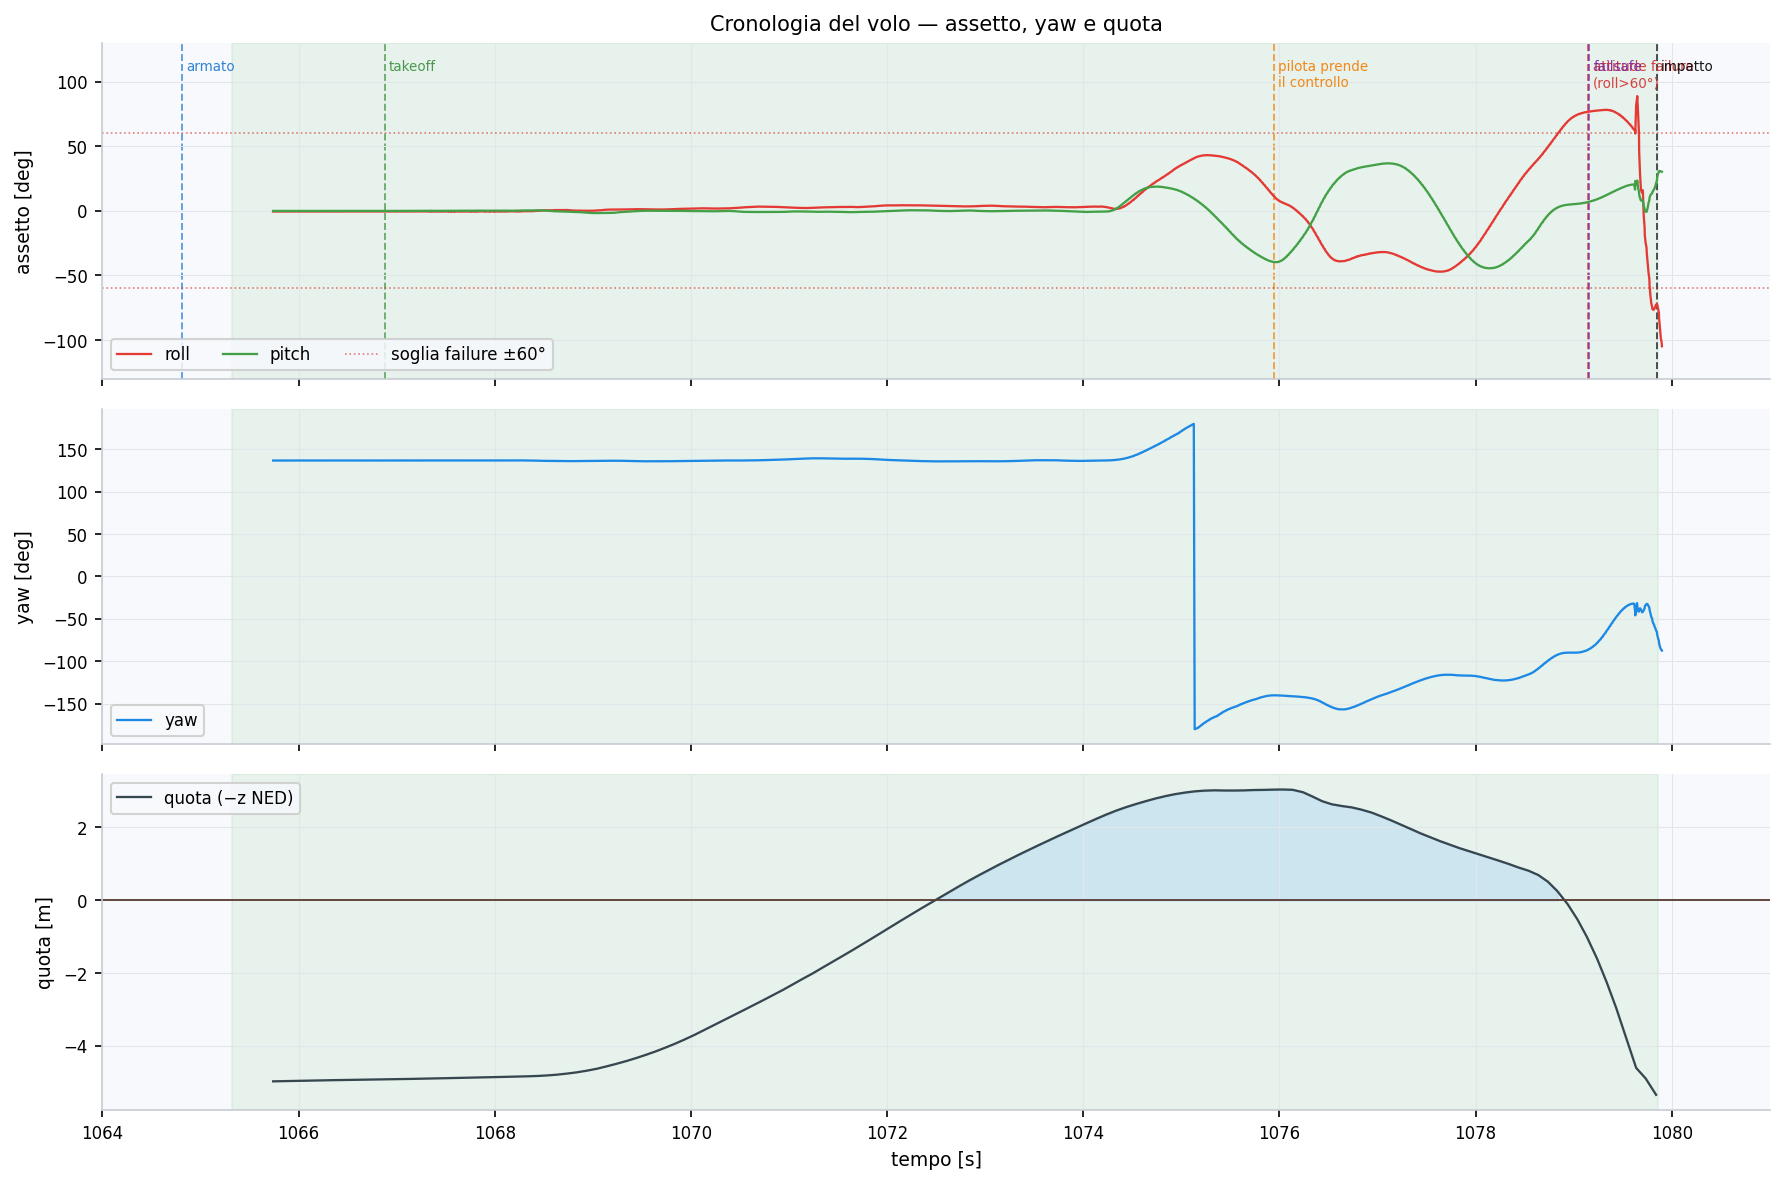
\includegraphics[width=0.92\linewidth]{cronologia_volo.png}
\caption{Cronologia dell'incidente: roll/pitch/yaw e quota con gli eventi
annotati (takeover, AUTO\_LAND, impatto).}
\label{fig:incidente-crono}
\end{figure}

\begin{figure}[H]
\centering
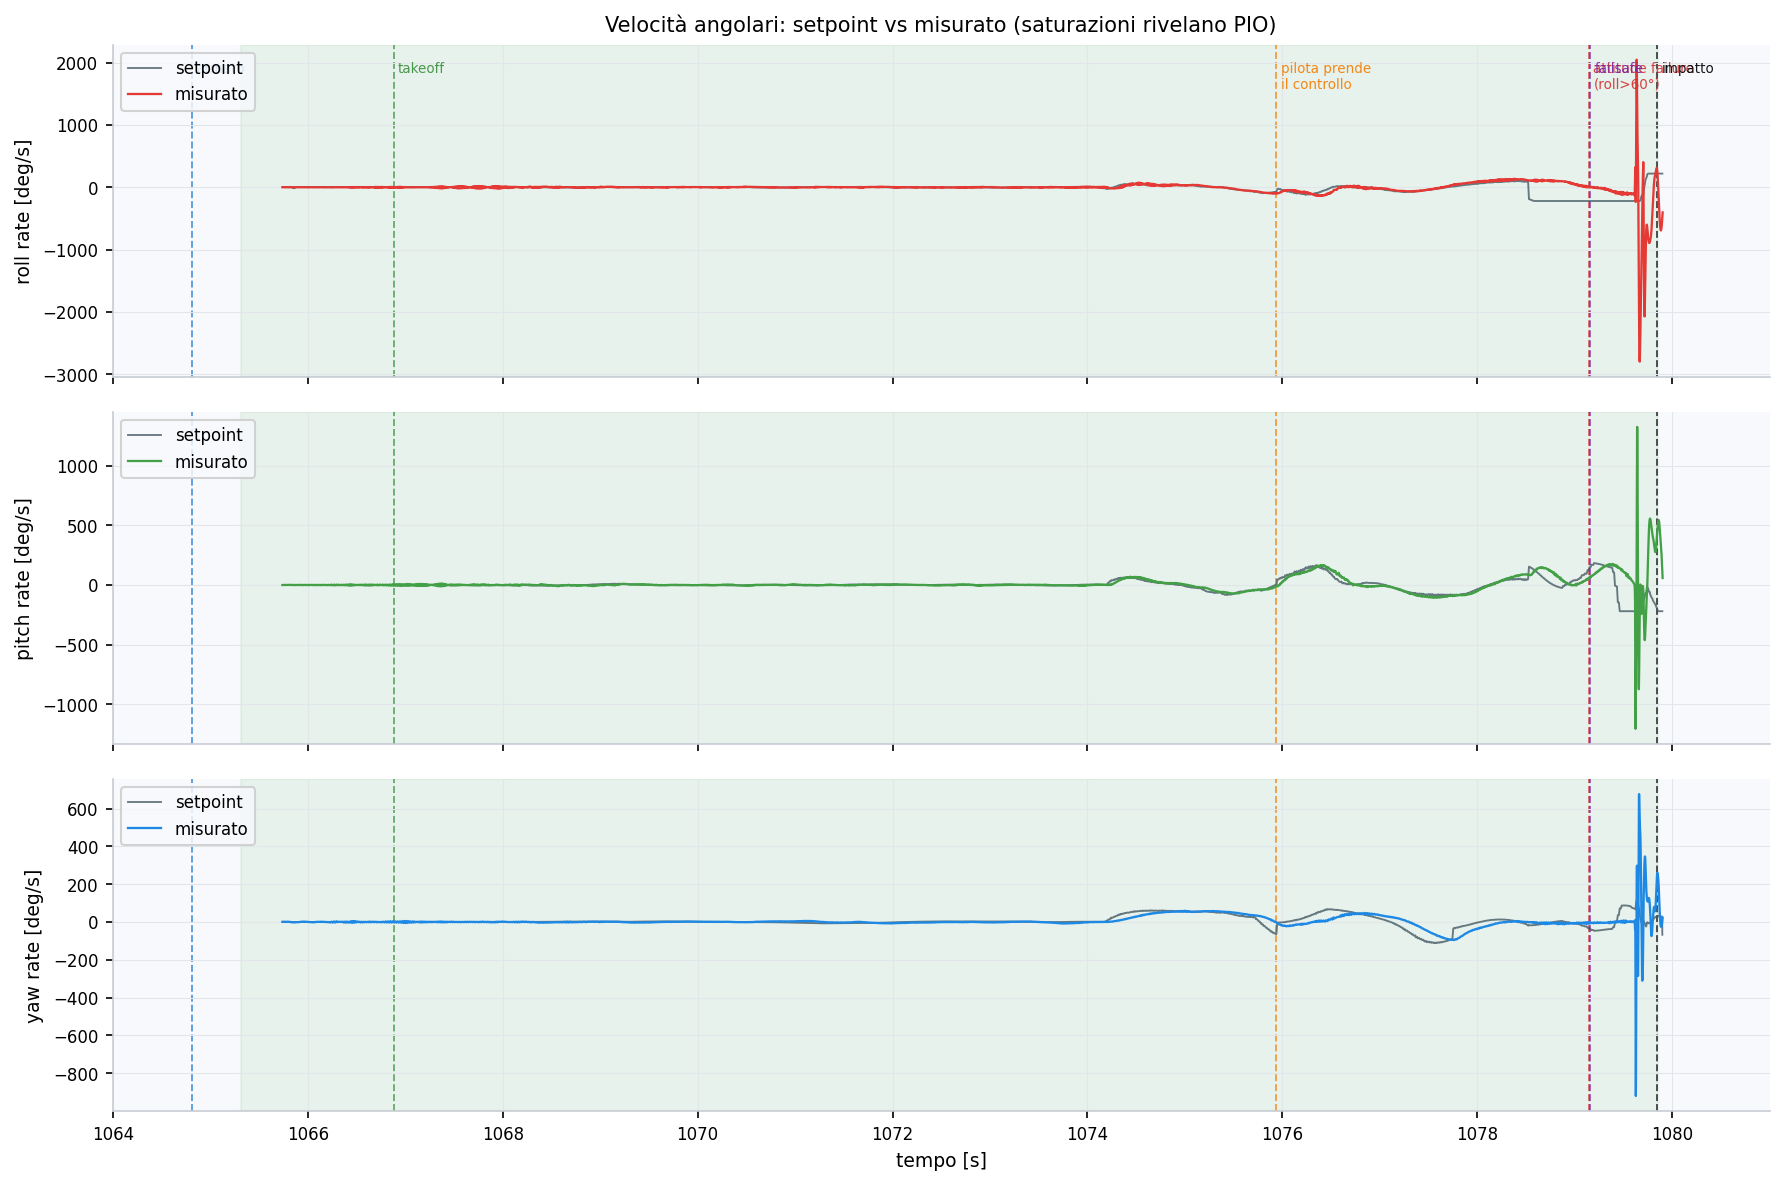
\includegraphics[width=0.92\linewidth]{dinamica_angolare.png}
\caption{Dinamica angolare: rate setpoint vs misurato sui tre assi. La
saturazione del rate ($\pm$220\textdegree/s) \`e la firma della PIO.}
\label{fig:incidente-dyn}
\end{figure}

Da questa analisi discendono alcune precauzioni operative concrete: portare lo
stick del throttle in posizione neutra \emph{prima} di ogni cambio di modo verso
POSCTL, preferire ALTCTL come modalit\`a di transizione, rivedere il tuning del
controllore di rate e verificare l'integrit\`a strutturale dopo ogni impatto.

\chapter{Osservazioni sui dati}
\label{cap:osservazioni}

\begin{notabox}[Capitolo non richiesto dal progetto]
Le analisi quantitative sui dati non erano un obiettivo del progetto (focalizzato
su messa in funzione e acquisizione). Si riportano qui in forma sintetica perch\'e
mostrano che i dati acquisiti sono effettivamente \emph{utili} alla diagnosi
dello stato di salute, chiudendo il filo conduttore della relazione.
\end{notabox}

\section{Metodo}

Per ogni log, sull'intervallo armato pi\`u lungo, sono state estratte metriche
scalari (vibrazione accelerometro e giroscopio, \texttt{imbalanced\_prop\_metric},
hover thrust) e metriche per-motore (RPM e comando normalizzato). Per queste
ultime si usa il \textbf{rapporto} tra il valore medio del motore $i$ e la media
degli altri cinque: un valore $>1$ indica che quel motore lavora pi\`u del gruppo.
Il confronto \`e fra Set A (baseline), Set B (5\,\%) e Set C (10\,\%) in hover.

\section{Vibrazione e squilibrio: baseline / 5\,\% / 10\,\%}

La Tabella~\ref{tab:confronto-danno} sintetizza il confronto trasversale. Due
risultati spiccano: (i) il danno al \textbf{5\,\% \`e quasi invisibile nelle
medie} e vive solo nei picchi; (ii) al \textbf{10\,\% tutte le metriche di
vibrazione raddoppiano}. La metrica con il miglior rapporto segnale/rumore \`e
\texttt{imbalanced\_prop\_metric} ($\times$2 al 5\,\%, $\times$6 al 10\,\%).

\begin{table}[H]
\centering
\caption{Metriche aggregate in hover: baseline vs pala 5\,\% vs pala 10\,\% (su M1).}
\label{tab:confronto-danno}
\small
\begin{tabularx}{\linewidth}{@{}L{5.4cm} r r r@{}}
\toprule
\textbf{Metrica} & \textbf{A (sane)} & \textbf{B (5\,\%)} & \textbf{C.1 (10\,\%)} \\
\midrule
\texttt{accel\_vib} mean (m/s\textsuperscript{2}) & 2{,}14 & 2{,}14 & \textbf{3{,}72} \\
\texttt{accel\_vib} max & 3{,}45 & 4{,}03 & \textbf{7{,}74} \\
\texttt{gyro\_vib} mean (rad/s) & 0{,}255 & 0{,}232 & \textbf{0{,}393} \\
\texttt{gyro\_vib} max & 0{,}387 & 0{,}442 & \textbf{0{,}836} \\
\texttt{imbalanced\_prop} p95 & $-$0{,}063 & $-$0{,}134 & \textbf{$-$0{,}358} \\
\texttt{hover\_thrust} mean & 0{,}525 & 0{,}513 & 0{,}555 \\
\bottomrule
\end{tabularx}
\end{table}

\begin{figure}[H]
\centering
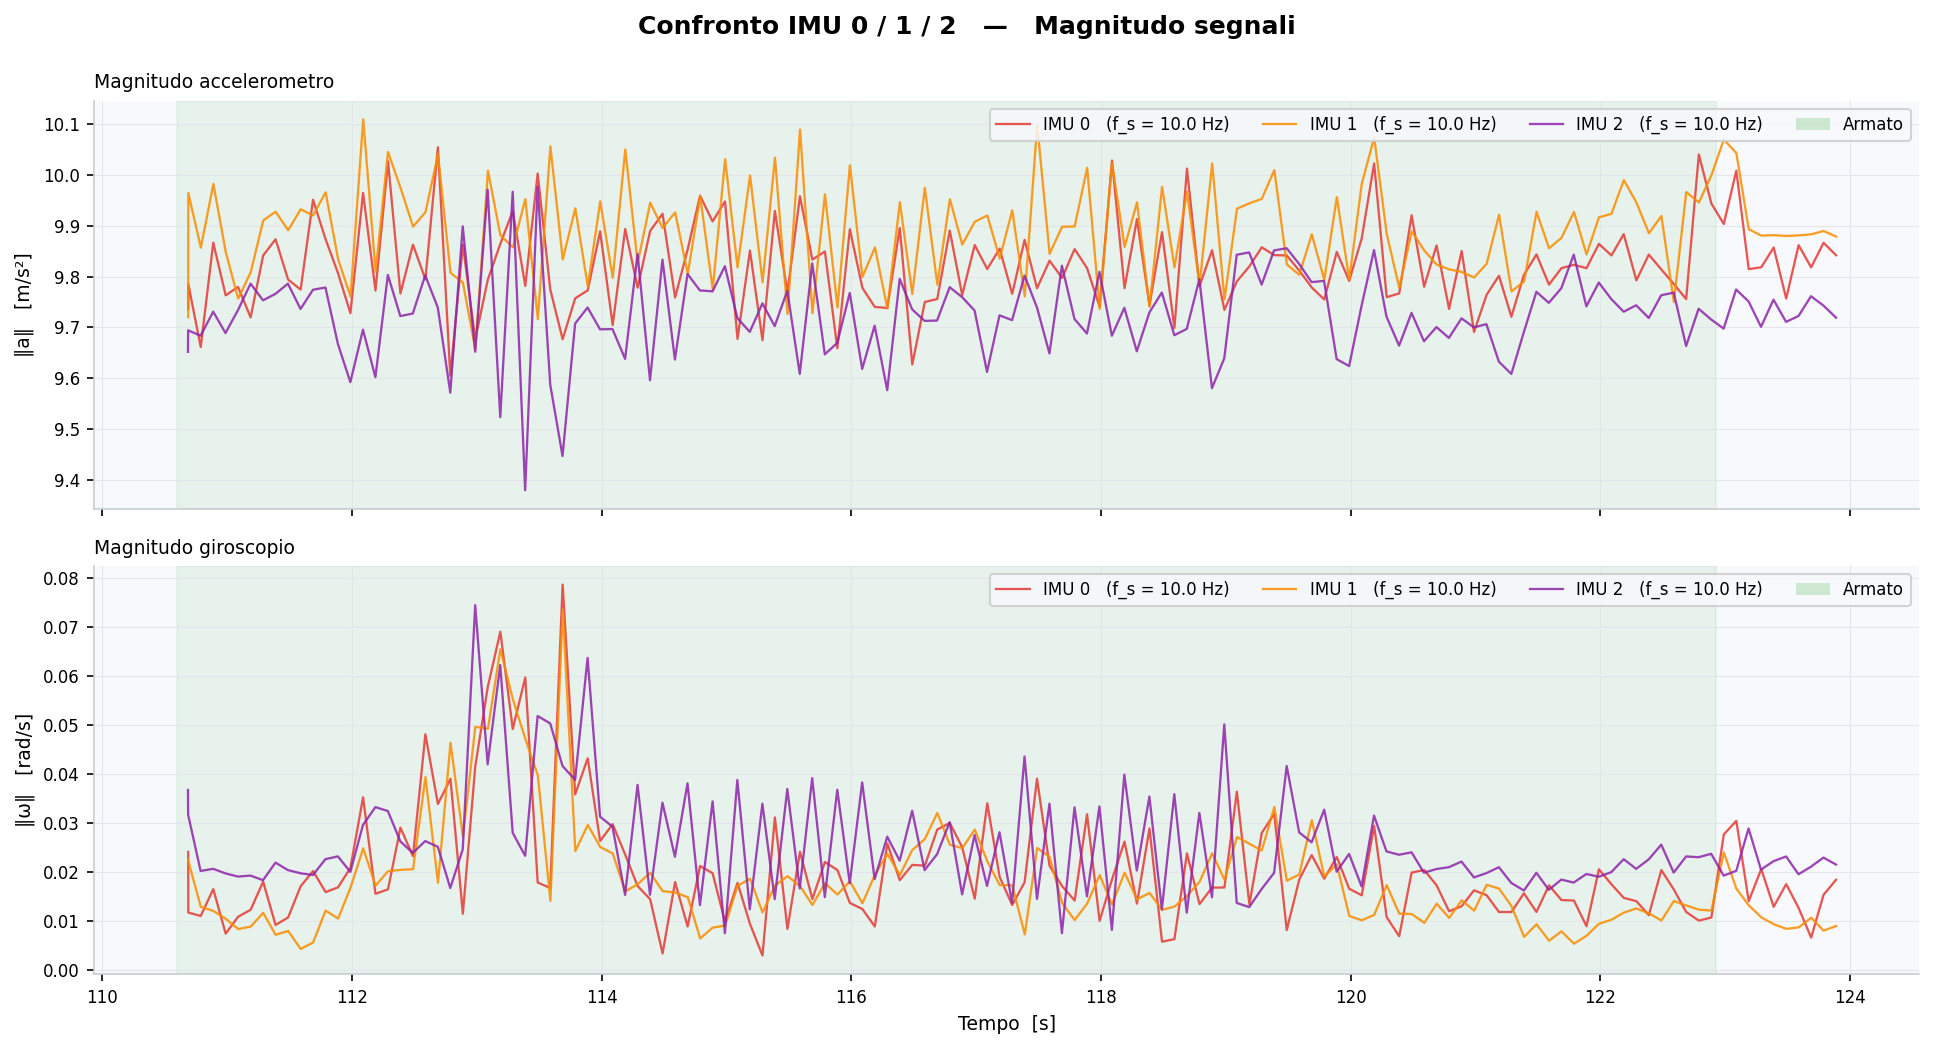
\includegraphics[width=0.95\linewidth]{imu_confronto.png}
\caption{Confronto delle firme vibrazionali tra le configurazioni di pala.}
\label{fig:imu-confronto}
\end{figure}

\section{Progressione monotona su M1}

Su M1 --- l'unico motore con tutti e tre i livelli di danno --- la firma \`e
\textbf{monotona e pulita} sia per il comando sia per gli RPM: il rapporto di
comando passa da 0{,}975 (sano) a 0{,}995 (5\,\%) a 1{,}014 (10\,\%). Il mixer
porta il motore dal sotto-comando strutturale al sopra-comando per compensare la
pala mancante. La progressione quasi lineare suggerisce che questo rapporto possa
fungere da \textbf{indicatore proxy del livello di danno} nell'intervallo
0--10\,\%.

\begin{figure}[H]
\centering
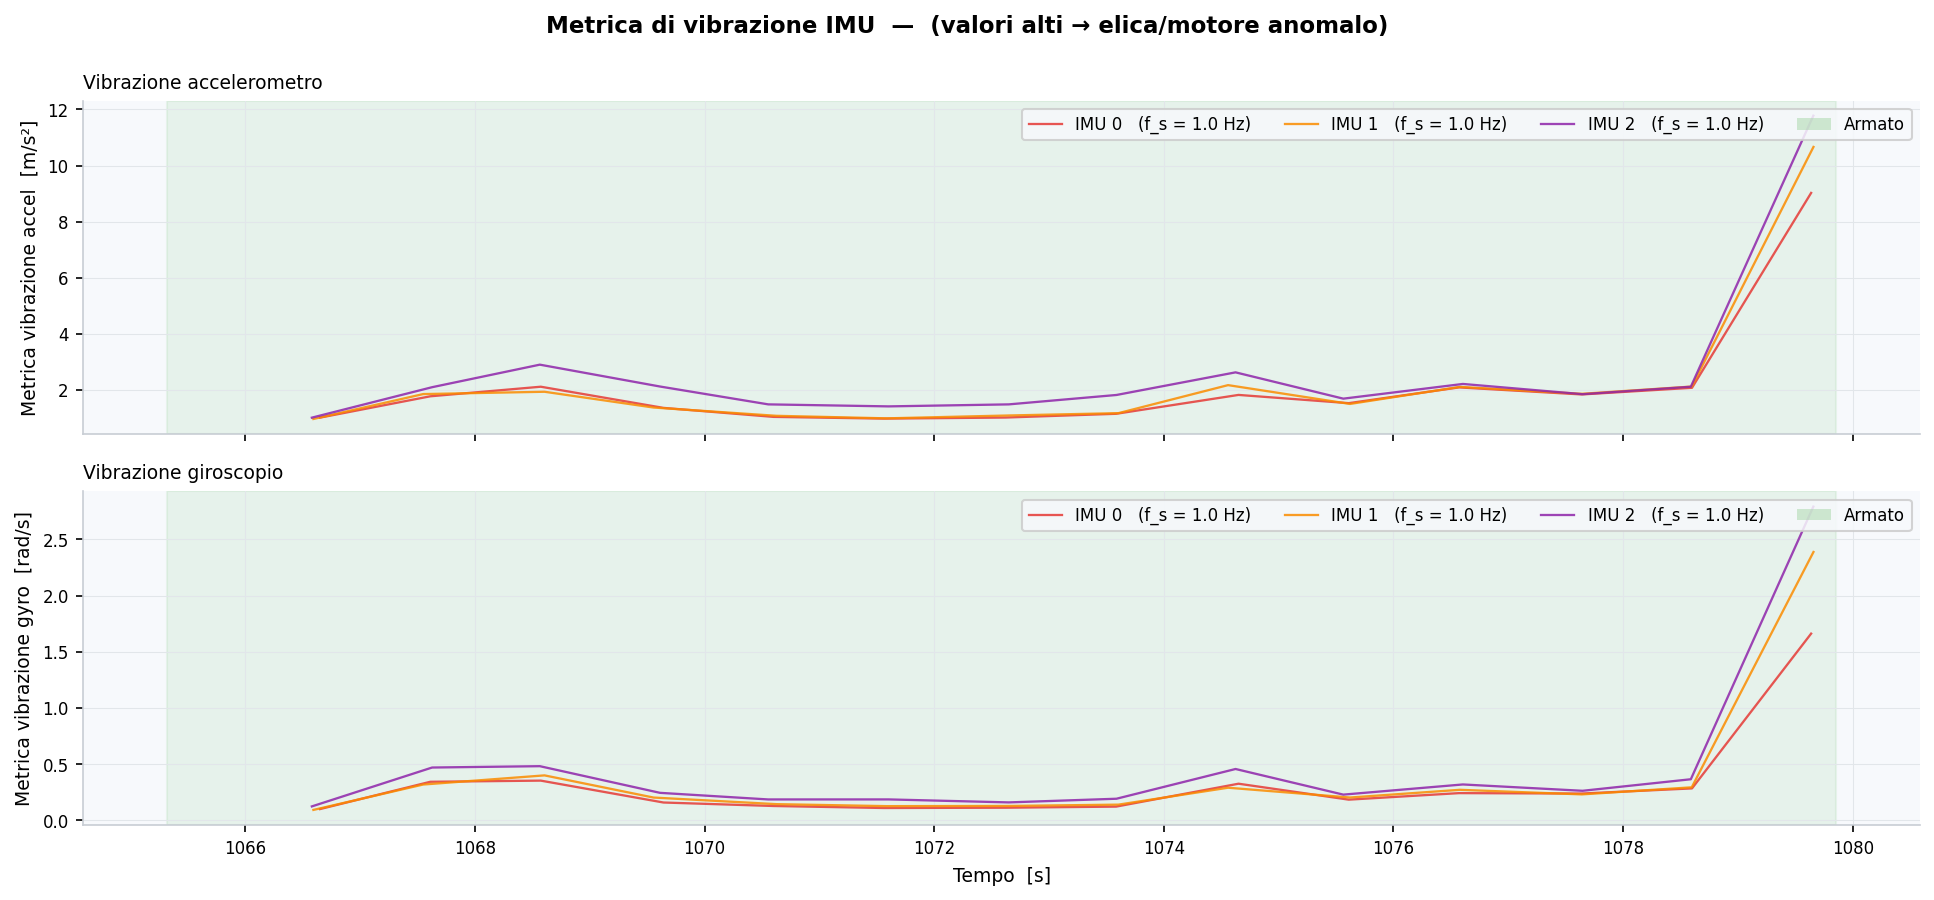
\includegraphics[width=0.95\linewidth]{imu_vibrazione.png}
\caption{Andamento temporale della metrica di vibrazione durante l'hover.}
\label{fig:imu-vibrazione}
\end{figure}

\section{Metriche raccomandate}

In ordine di rapporto segnale/rumore osservato nel range 0--10\,\%:
\texttt{imbalanced\_prop\_metric} p95, \texttt{accel\_vib} max, \texttt{gyro\_vib}
max e il rapporto comando/RPM del motore danneggiato (utile per stimare il
\emph{livello} di danno). Sono invece sconsigliate come metriche primarie
\texttt{hover\_thrust} e le \emph{medie} di vibrazione, dominate dalla scarica
batteria e dalla variabilit\`a inter-volo.

\chapter{Foxglove e interfaccia di visualizzazione}
\label{cap:foxglove}

\begin{notabox}[Contributo extra]
Lo strumento descritto qui non era previsto dal progetto: \`e stato realizzato per
comodit\`a di analisi (in particolare per l'indagine forense dell'incidente del
26/05) e si \`e rivelato utile per tutta la campagna. \`E presentato in fondo come
contributo aggiuntivo.
\end{notabox}

\section{Motivazione}

Gli script matplotlib (cartella \texttt{plot/}) sono ottimi per analisi mirate,
ma non danno una visione \emph{spazio-temporale} del volo. Per ricostruire
visivamente l'incidente serviva un replay 3D sincronizzato con la telemetria.
L'extension PX4 ufficiale di Foxglove si \`e rivelata inaffidabile sui nostri log
(alcuni topic, tra cui \texttt{vehicle\_attitude}, non venivano convertiti,
lasciando vuoto l'albero delle trasformate). La soluzione \`e stata una pipeline
custom che precompila tutto il necessario nel file di output.

\section{Pipeline \texttt{.ulg} $\rightarrow$ \texttt{.mcap}}

Lo script \texttt{foxglove/ulog\_to\_mcap.py} converte il log PX4 in un file
\texttt{.mcap} \textbf{autoconsistente} (nessun plugin richiesto in Foxglove).
Oltre a copiare i 147 topic uORB originali, lo script inietta i dati derivati
necessari al replay 3D:

\begin{itemize}
  \item le trasformate \texttt{/tf} corpo (\texttt{local\_origin}$\rightarrow$
        \texttt{base\_link}) con conversione di coordinate NED$\rightarrow$ENU e
        FRD$\rightarrow$FLU;
  \item le trasformate delle sei eliche, con angolo integrato dagli RPM di
        \texttt{esc\_status} e fattore di scala visivo (per evitare l'aliasing
        \emph{wagon-wheel});
  \item topic interpretativi (\texttt{attitude\_euler} in gradi,
        \texttt{flight\_state} con quota positivo-up e nomi leggibili dei modi di
        volo) e i \texttt{logged\_messages} del firmware.
\end{itemize}

\figurasegnaposto{Schema della pipeline \texttt{.ulg} $\rightarrow$
\texttt{.mcap} $\rightarrow$ Foxglove (topic uORB + transform + derivati).}{Schema
-- da generare}{fig:pipeline-mcap}

\section{Modello 3D e scena}

Il drone \`e rappresentato da un modello \textbf{URDF} puro
(\texttt{f550.urdf}), stilizzato ma fedele alle proporzioni dell'F550 (frame,
mast GPS, sei bracci con motori ed eliche), con i due bracci anteriori colorati
per indicare il fronte. La scelta dell'URDF rispetto a una mesh fotorealistica
privilegia riproducibilit\`a, manutenibilit\`a e leggibilit\`a tecnica. \`E
disponibile anche un \textbf{overlay satellitare} georeferenziato sul punto di
decollo (tile ESRI World Imagery), embeddato direttamente nel \texttt{.mcap}.

\section{Layout dei pannelli}

Il layout committato (\texttt{foxglove/drone f550.json}) organizza 9 pannelli in
due colonne: a sinistra la scena 3D con RPM motori, comandi mixer e input del
pilota; a destra i messaggi di log, le transizioni di stato di volo, la qualit\`a
del fix GPS e l'altitudine. Durante lo scrubbing si vede simultaneamente il drone
muoversi nello spazio e l'evoluzione di tutte le grandezze diagnostiche --- la
modalit\`a con cui \`e stata ricostruita la dinamica dell'incidente del
Capitolo~\ref{cap:diagnostici}.

\figurasegnaposto{Screenshot dell'interfaccia Foxglove realizzata: scena 3D con
modello URDF, overlay satellitare e pannelli di telemetria sincronizzati.}{Screenshot
-- da catturare, chiave}{fig:foxglove-ui}

\chapter{Conclusioni}
\label{cap:conclusioni}

Il progetto ha percorso l'intero arco previsto: \emph{mettere in funzione} il
drone, \emph{configurarlo} con QGroundControl e PX4, ed \emph{eseguire i test
acquisendo dati}. Al termine, l'esacottero F550 \`e un velivolo volabile e
pienamente strumentato, con una catena di acquisizione (147 topic uORB, FIFO
inerziali a $\sim$1\,kHz, telemetria ESC e batteria) adeguata alla diagnosi dello
stato di salute.

\section{Risultati principali}

\begin{itemize}
  \item \textbf{Sistema operativo e strumentato}: configurazione completa di
        sensori, GPS UART, power module, telemetria ESC, failsafe e profilo di
        logging.
  \item \textbf{Campagna di volo conclusa}: hover baseline e con pala 5\,\%/10\,\%
        (Set A--C), traiettorie quadrate 5\,\%/10\,\% (Set D--E) e un blocco extra
        con payload (Set P).
  \item \textbf{Guasti diagnosticati e risolti}: dalla sostituzione del flight
        controller alla ricostruzione del cavo GPS (ri-crimpatura e schermatura),
        che ha eliminato il contatto meccanico intermittente responsabile dei
        dropout (BER 49\,\%\,$\rightarrow$\,0{,}24\,\%); resta aperto, come secondo
        modo di guasto indipendente, lo stallo del driver GPS in modo RTK, per cui
        la campagna \`e stata condotta in GPS standard. Ogni caso \`e stato
        documentato con la sua diagnosi e azione correttiva.
  \item \textbf{Dati utili}: le metriche estratte (vibrazione,
        \texttt{imbalanced\_prop}, rapporto comando/RPM) discriminano il livello
        di danno alla pala, confermando la bont\`a dell'acquisizione.
  \item \textbf{Contributo extra}: una pipeline di visualizzazione 3D in Foxglove
        per il replay dei voli.
\end{itemize}

\section{Limiti e sviluppi futuri}

La campagna non comprende le traiettorie casuali (Set F/G), non eseguite, n\'e le
prove al 15\,\% (sospese dal docente). Il bias strutturale di montaggio
(M3/M6 vs M4/M5) andrebbe caratterizzato e corretto prima di estendere le analisi
alle traiettorie. Sul fronte hardware, la ridondanza GPS (secondo modulo M9N) e
l'upgrade a un ricevitore multi-banda (ZED-F9P) migliorerebbero robustezza e
precisione RTK. Infine, le analisi del Capitolo~\ref{cap:osservazioni} possono
essere estese con un'analisi FFT sistematica dei FIFO inerziali per legare le
firme spettrali al tipo e al livello di danno.


% --------------------------- APPENDICI ---------------------------
\appendix
\chapter{Appendici}
\label{cap:appendici}

Le appendici raccolgono i dettagli fini richiamati dai capitoli ma tenuti fuori
dal corpo principale per leggibilit\`a.

\section{Mappatura dei log per sessione}

Le tabelle seguenti mappano i file \texttt{.ulg} alle prove del piano voli. Il
dettaglio completo (tensioni di batteria, voli di riscaldamento e ripetizioni per
batteria scarica) \`e nei file \texttt{log/<data>/README.md} del repository.

\begin{table}[H]
\centering
\caption{Set A--C --- hover (27/05 e 04/06). Pala a turno su M1\ldots M6.}
\label{tab:app-abc}
\scriptsize
\begin{tabularx}{\linewidth}{@{}c L{4.0cm} l@{}}
\toprule
\textbf{Prova} & \textbf{Configurazione} & \textbf{Log} \\
\midrule
A.1--A.6 & Pale sane (swap coppie) & \texttt{2026-05-27/13\_56\_40 \ldots 14\_15\_52} \\
\addlinespace
B.1 & Pala 5\,\% su M1 & \texttt{2026-05-27/16\_00\_57} \\
B.2 & Pala 5\,\% su M2 & \texttt{2026-05-27/15\_47\_35} \\
B.3 & Pala 5\,\% su M3 & \texttt{2026-05-27/16\_03\_10} \\
B.4 & Pala 5\,\% su M4 & \texttt{2026-05-27/15\_50\_20} \\
B.5 & Pala 5\,\% su M5 & \texttt{2026-05-27/15\_54\_10} \\
B.6 & Pala 5\,\% su M6 & \texttt{2026-05-27/16\_05\_24} \\
\addlinespace
C.1 & Pala 10\,\% su M1 & \texttt{2026-05-27/16\_07\_29} \\
C.2 & Pala 10\,\% su M2 & \texttt{2026-06-04/12\_39\_37} \\
C.3 & Pala 10\,\% su M3 & \texttt{2026-06-04/12\_21\_42} \\
C.4 & Pala 10\,\% su M4 & \texttt{2026-06-04/12\_43\_47} \\
C.5 & Pala 10\,\% su M5 & \texttt{2026-06-04/12\_46\_09} \\
C.6 & Pala 10\,\% su M6 & \texttt{2026-06-04/12\_28\_29} \\
\bottomrule
\end{tabularx}
\end{table}

\begin{table}[H]
\centering
\caption{Set D ed E --- quadrato 8$\times$8\,m. Il baseline pale sane \`e condiviso
(\texttt{13\_21\_21}).}
\label{tab:app-de}
\scriptsize
\begin{tabularx}{\linewidth}{@{}c l c l@{}}
\toprule
\textbf{Prova} & \textbf{Log (Set D, 5\,\%)} & \textbf{Prova} & \textbf{Log (Set E, 10\,\%)} \\
\midrule
D.1 (sane) & \texttt{2026-06-05/13\_21\_21} & E.1/E.2 & riusa D.1 \\
D.3/D.4 (M1) & \texttt{13\_25\_30 / 13\_32\_25} & E.3/E.4 (M1) & \texttt{13\_27\_52 / 13\_33\_16} \\
D.5/D.6 (M2) & \texttt{14\_08\_33 / 14\_11\_02} & E.5/E.6 (M2) & \texttt{13\_52\_09 / 13\_59\_52} \\
D.7/D.8 (M3) & \texttt{13\_37\_21 / 13\_40\_36} & E.7/E.8 (M3) & \texttt{13\_37\_29 / 13\_40\_32} \\
D.9/D.10 (M4) & \texttt{14\_17\_24 / 14\_34\_05} & E.9/E.10 (M4) & \texttt{14\_15\_24 / 14\_18\_32} \\
D.11 (M5) & \texttt{2026-06-12/13\_20\_00} & E.11/E.12 (M5) & \texttt{14\_06\_38 / 14\_09\_45} \\
D.13/D.14 (M6) & \texttt{13\_45\_18 / 14\_05\_24} & E.13/E.14 (M6) & \texttt{13\_44\_15 / 13\_47\_50} \\
\bottomrule
\end{tabularx}
\end{table}

\begin{table}[H]
\centering
\caption{Set P --- payload (12/06, blocco extra fuori piano A--G).}
\label{tab:app-p}
\scriptsize
\begin{tabularx}{\linewidth}{@{}c L{4.4cm} l l@{}}
\toprule
\textbf{Prova} & \textbf{Configurazione} & \textbf{Traiettoria} & \textbf{Log} \\
\midrule
P.1 & Payload, pale sane & libera & \texttt{2026-06-12/14\_44\_38} \\
P.2 & Payload, pale sane & libera & \texttt{2026-06-12/14\_50\_12} \\
P.3 & Payload, pala 10\,\% M2 & quadrato & \texttt{2026-06-12/15\_29\_08} \\
P.4 & Payload, pala 10\,\% M2 & quadrato & \texttt{2026-06-12/15\_31\_52} \\
P.5 & Payload, pala 5\,\% M2 & quadrato & \texttt{2026-06-12/15\_35\_21} \\
\bottomrule
\end{tabularx}
\end{table}

\section{Parametri PX4 rilevanti}

\begin{table}[H]
\centering
\caption{Parametri PX4 principali configurati durante il progetto.}
\label{tab:app-param}
\small
\begin{tabularx}{\linewidth}{@{}l l L{6.4cm}@{}}
\toprule
\textbf{Parametro} & \textbf{Valore} & \textbf{Funzione} \\
\midrule
\texttt{UAVCAN\_ENABLE} & 0 & Disabilita DroneCAN (GPS su UART) \\
\texttt{GPS\_1\_CONFIG} & 202 & GPS su porta GPS\,2 \\
\texttt{GPS\_DUMP\_COMM} & 1 & Dump UART grezzo per diagnosi (poi disattivabile) \\
\texttt{BAT1\_V\_CHANNEL} & 16 & Canale ADC tensione batteria \\
\texttt{BAT1\_I\_CHANNEL} & 17 & Canale ADC corrente batteria \\
\texttt{DSHOT\_CONFIG} & 600 & DShot600 verso gli ESC \\
\texttt{DSHOT\_TEL\_CFG} & 102 & Telemetria ESC su TELEM2 \\
\texttt{SDLOG\_PROFILE} & 849 & Profilo di logging (default+HF+3IMU+FIFO) \\
\texttt{IMU\_GYRO\_RATEMAX} & 1000 & Frequenza massima giroscopio (Hz) \\
\texttt{EKF2\_NOAID\_TOUT} & 10\,s & Timeout EKF perdita posizione \\
\texttt{COM\_POSCTL\_NAVL} & Altitude & Failsafe perdita posizione in POSCTL \\
\texttt{MPC\_XY\_VEL\_MAX} & 5\,m/s & Velocit\`a orizzontale massima \\
\texttt{MPC\_TILTMAX\_AIR} & 25\textdegree & Tilt massimo in volo \\
\bottomrule
\end{tabularx}
\end{table}

\section{Riferimenti al repository}

I documenti di dettaglio sono mantenuti nel repository di progetto:
\texttt{diario.md} (cronologia), \texttt{piano-voli.md} (piano completo),
\texttt{docs/BOM.md} (BOM), \texttt{maintenance/} (troubleshooting e checklist),
\texttt{analisi/} (analisi pale), \texttt{plot/} (script e grafici),
\texttt{foxglove/} (pipeline di visualizzazione).


\end{document}
